% --- Documentclass specifications ---
\documentclass[italian]{tktltiki2}
\linespread{1.3}

% --- General packages ---
\usepackage[utf8]{inputenc}
\usepackage[T1]{fontenc}
\usepackage{lmodern}
\usepackage{float}
\usepackage{epigraph}
\usepackage{microtype}
\usepackage{amsfonts,amsmath,amssymb,amsthm,booktabs,color,enumitem,graphicx}
\usepackage[pdftex,hidelinks]{hyperref}
% setting C language style listing
\usepackage{listings}
\lstset{language=C,
  basicstyle=\fontsize{8}{11}\selectfont\ttfamily,  
  breaklines=true,
  numberstyle=\tiny,
  numbers=left,
  keywordstyle=\color{blue}\ttfamily,
  stringstyle=\color{red}\ttfamily,
  commentstyle=\color{magenta}\ttfamily,
  morecomment=[l][\color{magenta}]{\#}
}
% Automatically set the PDF metadata fields
\makeatletter
\AtBeginDocument{\hypersetup{pdftitle = {\@title}, pdfauthor = {\@author}}}
\makeatother

% --- Language-related settings ---
\usepackage[fixlanguage]{babelbib}
% add bibliography to the table of contents
\usepackage[nottoc]{tocbibind}

% --- tktltiki2 options ---
%
% The following commands define the information used to generate title and
% abstract pages. The following entries should be always specified:
\title{%
    \huge Project Heimdall 
    \\
    \large Proposta di implementazione per un web switch 
    \\
    concorrente two-way di livello 7 (OSI) con
    \\
    politiche di bilanciamento del carico state less e state aware
  }
  \author{\emph{Alessio Moretti} - 0187698
    \\
    \emph{Andrea Cerra} - 0167043
    \\
    \emph{Claudio Pastorini} - 0186256}
  \date{\today}
  \level{Corso di Ingegneria di Internet e del Web - A.A. 2014/2015}
  \university{\textbf{Università degli studi di Roma Tor Vergata}}
  \department{\textbf{Facoltà di Ingegneria Informatica}}
  \city{Roma}

\begin{document}

% --- Front matter ---
\maketitle        % title page

\tableofcontents  % table of contents
\pagenumbering{gobble}

% --- Main matter ---
\mainmatter       % clear page, start arabic page numbering

\thispagestyle{empty} 
\begin{figure}[H]
\centering

\includegraphics[width=\textwidth]{images/heimdall}
\caption{Heimdall guardiano del \emph{Bifröst} e del \emph{regno di Asgard}}
\end{figure}

% --- Main matter ---
\pagenumbering{gobble}
\mainmatter       % clear page, start arabic page numbering
\newpage
\section{Introduzione}
\subsection{Perché Heimdall?}
Heimdall è un personaggio dell'universo Marvel, ispirato all'omonimo dio della mitologia norrena, egli è il guardiano del regno di Asgard e del Bifröst. Quest'ultimo è il ponte che unisce la Terra alla dimora degli dei ed Heimdall, come suo custode, ha il compito di aprirlo ed indirizzarlo verso gli altri mondi, permettendo solamente a chi è degno di attraversare le distese dello spazio.
\\
Ci piace pensare che questo sia un po' il ruolo del software nato dal nostro progetto: che sia in grado di scegliere come meglio indirizzare le connessioni in arrivo, ponendosi come ``guardiano'' di un cluster di server che fa ad esso capo. Quindi un \textbf{web switch} che sia funzionale sia per ricevere o trasmettere pacchetti di un regolare traffico HTTP, che per bilanciare il carico dello stesso traffico in arrivo sulle varie macchine.

\subsection{Web switch di livello 7}
Nella terminologia delle reti informatiche uno \textbf{switch} è un commutatore a livello datalink, ovvero un dispositivo che si occupa di instradare opportunamente, attraverso le reti LAN, selezionando i frame ricevuti e reindirizzandoli verso la macchina appropriata a seconda di una propria tabella di inoltro. Un \textbf{web switch}, a livello applicativo, è capace di reindirizzare i dati in funzione dei pacchetti che riceve, analizzandone il contenuto e decidendo opportunamente la destinazione, occupandosi allo stesso tempo di reinoltrare anche l'eventuale risposta della macchina selezionata verso il client che l'ha generata.
\\
Le applicazioni sono molteplici per l'implementazione a livello applicativo: può essere considerato un \textbf{proxy}, oppure, selezionando opportunamente la macchina con più velocità di risposta o con minore pressione, può agire come \textbf{bilanciatore di carico}. Infatti ognuno dei client che fa richiesta, ad esempio, per uno specifico sito web, invia un pacchetto ad un indirizzo IP pubblico che corrisponde a quello del nostro switch applicativo. Questi, dopo aver correttamente letto il pacchetto, si occupa di consultare una tabella di inoltro generata con una determinata \textbf{politica di scheduling} e quindi gestire l'inoltro della richiesta ed il reinoltro della risposta del web server. Tutto questo in maniera totalmente trasparente al client.

\subsection{Assunzioni progettuali sul cluster}
Nella fase di progettazione e realizzazione sono state definite le seguenti assunzioni:
\begin{itemize}
  \item Ognuna delle macchine del cluster dispone di un web server Apache\cite{apache_server} in ascolto sulla porta 80;
  \item Ognuna delle macchine monta il modulo ApacheStatus (\ref{sssec:apachestatus}) come monitor di carico.
\end{itemize}

\begin{figure}
\centering
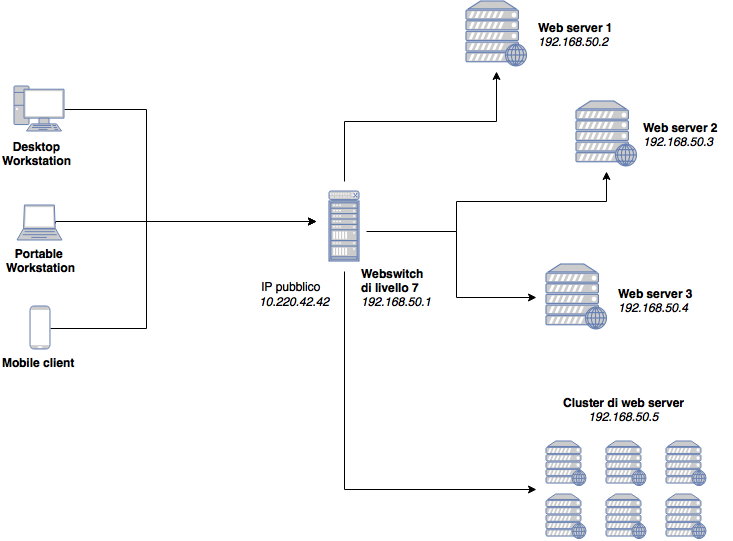
\includegraphics[width=\textwidth]{images/switch7}
\caption{Esempio di uno \emph{switch di livello 7 (OSI)}}
\end{figure}

\newpage
\section{Architettura}
\label{sec:architecture}

\subsection{Overview}
\label{ssec:overview}

\subsection{Il processo principale}
\label{ssec:main_process}
Il cuore di Heimdall è codificato nel \emph{main.c} da cui inizia l'esecuzione del processo principale.
\\
Il processo, una volta avviato, inizializzerà i componenti principali, tra questi abbiamo:

\begin{itemize}
  \item Config (paragrafo \ref{sec:config});
  \item Log (paragrafo \ref{ssec:logging});
  \item Scheduler (paragrafo \ref{ssec: sched});
  \item Pool Manager (paragrafo \ref{ssec:pool}).
\end{itemize}
Possiamo dividere questi quattro componenti in due categorie, i primi due infatti sono semplici strutture statiche all'interno del programma, sviluppate utilizzando il design pattern \emph{Singleton}. Questo per garantire che questi due componenti vengano inizializzati una sola volta all'avvio del programma. I successivi due componenti, lo \emph{Scheduler} e il \emph{Pool Manager} sono invece thread del processo principale, questo perché (come sarà più chiaro nei relativi paragrafi) svolgono alcuni compiti dedicati che altrimenti dovrebbero essere eseguiti dal processo principale.

\subsubsection{I processi figli e la memoria condivisa}
\label{ssec:child_process}

Fatte le prime inizializzazioni, il processo principale si predispone ad eseguire il suo compito. Prima di questo, è necessario creare i processi figli che saranno incaricati di servire le connessioni HTTP. Tramite la funzione \emph{do\_prefork()}, presente nel file \emph{main.c}, il processo principale esegue una serie di operazioni per creare i processi figli e inizializzare una memoria condivisa, che verrà utilizzata per fornire l'\textbf{IPC} (\emph{Inter-Process Communication}). Per motivi che saranno più chiari in seguito, chiameremo da adesso in poi i processi figli \emph{Worker}. \\\\Evidenziamo qui i tratti principali della funzione:
\begin{lstlisting}
ConfigPtr config = get_config();

int n_prefork = 0;
ThrowablePtr throwable = str_to_int(config->pre_fork, &n_prefork);
if (throwable->is_an_error(throwable)) {
  get_log()->t(throwable);
}
\end{lstlisting}
Dal Config viene recuperato il numero di processi figli da creare e, come verrà spiegato nel paragrafo relativo, questo valore potrà essere specificato dall'utente all'interno del file di configurazione. Con questo parametro, oltre ad eseguire un numero finito di volte la chiamata di sistema \emph{fork()}, viene inizializzato un blocco di memoria condivisa di grandezza fissa, all'interno del quale vengono salvati quattro array che ora vedremo nel dettaglio:

\begin{itemize}
  \item \textbf{\emph{worker\_array}}: Array in cui vengono memorizzati i \emph{pid\_t} dei Worker.          
  \item \textbf{\emph{worker\_busy}}: Array di flag e viene utilizzato per tenere traccia dello stato del lavoro di un Worker. Nello specifico alla posizione i-esima, che viene identificata a partire dal primo array, possiamo trovare due valori distinti, un 1 per indicare che il Worker è occupato a gestire una connessione e uno 0 per indicare che il Worker è libero in attesa di nuove connessioni.
  \item \textbf{\emph{worker\_counter}}: Array che tiene traccia di quante connessioni sono state assegnate al Worker. Tale parametro sarà chiarito nel paragrafo del Pool Manager e servirà alla schedulazione dei Worker.
  \item \textbf{\emph{worker\_server}} \label{ssec:shm_server} : Struttura di passaggio utilizzata dal thread Scheduler, che ricordiamo essere uno dei componenti inizializzati all'avvio di Heimdall, la cui funzionalità sarà descritta in maniera più adeguata nel relativo paragrafo.
\end{itemize}
La seguente porzione di codice mette in evidenza le righe che si occupano della creazione, della mappatura e dell'inizializzazione della memoria condivisa.
\begin{lstlisting}
int total_size = 0;
total_size += sizeof(THPSharedMem);
total_size += sizeof(pid_t)*n_prefork;  // Array worker
total_size += sizeof(int)*n_prefork;    // Array busy
total_size += sizeof(int)*n_prefork;    // Array counter
total_size += sizeof(Server)*n_prefork; // Array server

// Initializes shared memory
void *start_mem = init_shm(WRK_SHM_PATH, total_size, WRK_SEM_PATH);
if (start_mem == NULL)
  exit(EXIT_FAILURE);

// Mapping shared memory segment
THPSharedMemPtr worker_pool = start_mem;
worker_pool->worker_array   = start_mem+sizeof(THPSharedMem);
worker_pool->worker_busy    = start_mem+sizeof(THPSharedMem)+sizeof(pid_t)*n_prefork;
worker_pool->worker_counter = start_mem+sizeof(THPSharedMem)+sizeof(pid_t)*n_prefork+sizeof(int)*n_prefork;
worker_pool->worker_server  = start_mem+sizeof(THPSharedMem)+sizeof(pid_t)*n_prefork+sizeof(int)*n_prefork+sizeof(int)*n_prefork;

int i = 0;
for (i = 0; i < n_prefork; ++i) {
  worker_pool->worker_counter[i]  = 0;
  worker_pool->worker_array[i]    = 0;
  worker_pool->worker_busy[i]     = 0;
}
\end{lstlisting}
La memoria condivisa utilizzata è quella appartenente allo standard POSIX, l'implementazione della wrapper proprietaria \emph{init\_shm()} è presente all'interno dei file \emph{shared\_mem.c} e \emph{shared\_mem.h}.
\\
\\
Siamo finalmente giunti alla creazione dei processi figli, i cosidetti Worker, ancora una volta evidenziamo qui la porzione di codice interessata:

\begin{lstlisting}
int children;
for (children = 0; children < n_prefork; ++children) {
  pid_t child_pid;
  errno = 0;

  child_pid = fork();
  if (child_pid == -1) {
    get_log()->t(get_throwable()->create(STATUS_ERROR, get_error_by_errno(errno), "do_prefork"));
  }
  // Child 
  if (child_pid == 0) {
    // see worker.c
    start_worker();
    break;
  } else {
    if (sem_wait(sem) == -1) {
      return get_throwable()->create(STATUS_ERROR, "sem_wait", "do_prefork");
    }
    // Scan array and set worker to first position available
    int i, flag = 0;
    for (i = 0; i < n_prefork; ++i) {
      if (worker_pool->worker_array[i] == 0) {
        worker_pool->worker_array[i] = child_pid;
        flag = 1;
        break;
      }
    }

    if (sem_post(sem) == -1) {
      return get_throwable()->create(STATUS_ERROR, "sem_post", "do_prefork");
    }

    if (flag == 0) {
      return get_throwable()->create(STATUS_ERROR, "Cannot add worker_pid to array", "do_prefork");        
    }            
  }
}
\end{lstlisting}
Nel codice sopraesposto, viene eseguito un ciclo \emph{n\_prefork} volte, dove \emph{n\_prefork} è il numero di processi che si vuole creare. Il Worker, una volta creato, si avvia eseguendo la funzione \emph{start\_worker()}; il processo padre invece si occupa di accedere in memoria condivisa per aggiornare le strutture dati che abbiamo spiegato sopra. \\\\Si noti, che l'esecuzione della chiamata di sistema \emph{fork()}, non viene casualmente eseguita in questo momento, bensì si sfrutta il fatto che la \emph{fork()} copia l'intera memoria del processo padre nella memoria del figlio e, grazie a questo il figlio si ritroverà i componenti come \emph{Config}, \emph{Log} e \emph{Memoria Condivisa} già inizializzati e referenziati.

\subsubsection{Server in ascolto}
\label{sec:main_server}
Una volta completata l'inizializzazione dei componenti di base di Heimdall, il processo principale si avvia a svolgere il suo incarico cioè quello di mettersi in ascolto su una porta (configurabile nel file di configurazione) in attesa di nuove connessioni.
\begin{lstlisting}
int port = 0;
throwable = str_to_int(config->server_main_port, &port);
if (throwable->is_an_error(throwable)) {
  log->t(throwable);
}

// Creates a new server
int sockfd;
throwable = create_server_socket(TCP, port, &sockfd);
if (throwable->is_an_error(throwable)) {
  log->t(throwable);
  exit(EXIT_FAILURE);
} 

log->i(TAG_MAIN, "Created new server that is listening on port %d", port);

// Starts listening for the clients
int backlog = 0;
throwable = str_to_int(config->backlog, &backlog);
if (throwable->is_an_error(throwable)) {
  log->t(throwable);
}

throwable = listen_to(sockfd, backlog);
if (throwable->is_an_error(throwable)) {
  log->t(throwable);
  exit(EXIT_FAILURE);
} 

log->i(TAG_MAIN, "Ready to accept incoming connections...");

int count = 0;

// Starts to listen incoming connections
while(TRUE) {
  // Accepts new connection
  int new_sockfd;
  throwable = accept_connection(sockfd, &new_sockfd);
  count++;
  if (throwable->is_an_error(throwable)) {
    log->t(throwable);
    exit(EXIT_FAILURE);
  }

  while(TRUE) {
    throwable = th_pool->add_fd_to_array(&new_sockfd);
    if (throwable->is_an_error(throwable)) {
      throwable->destroy(throwable);
    } else {
      break;
    }
  }

  log->i(TAG_MAIN, "New connection accepted on socket number %d - total %d", new_sockfd, count);
}
\end{lstlisting}
Questo è il vero cuore di Heimdall. Si noti che, da queste poche righe, il processo principale recupera dal config la porta dove mettersi in ascolto, crea un nuovo "\emph{server socket}" e si mette in attesa dell'arrivo di nuove connessioni in un loop infinito. Quando un nuovo client si collega la funzione \emph{accept\_connection()} ritorna e il processo principale prosegue la sua strada. Si noti che lo sviluppo della funzione \emph{main()} è stato pensato per poter eseguire il minor numero di linee di codice, per permettere al processo principale di tornare immediatamente in ascolto di nuove connessioni. Infatti, dopo aver salvato il file descriptor della socket in una apposita struttura dati (che sarà descritta nel paragrafo relativo al Pool Manager), il processo principale termina il primo ciclo del loop infinito e torna in ascolto di nuove connessioni. Come ultima cosa si sottolinea il fatto che l'esecuzione della chiamata \emph{fork()} viene eseguita prima dell'avvio del "server in ascolto", questo per evitare di dover attendere i lunghi tempi di fork.

\subsection{File di configurazione}
\label{sec:config}
I file di configurazione sono gli unici file accessibili all'utente che installa sulla propria macchina Heimdall WebSwitch. Tramite questi file è possibile impostare alcuni parametri per adattare il Web Switch alle proprie esigenze.
\\
\\
I file di cui stiamo parlando sono due e adesso ne illustreremo i dettagli.
\subsubsection{File dei parametri}
\label{sec:config_parser}
Questo è il file di configurazione generale di Heimdall. Al suo interno possiamo trovare i seguenti parametri:

\begin{itemize}
	\item \emph{algorithm\_selection}: specifica il tipo di algoritmo che si vuole usare per Heimdall, con il valore 0 si sceglie di usare l'algoritmo \emph{state-less}, con il valore 1 si sceglie di usare l'algoritmo \emph{state-aware}.

	\item \emph{pre\_fork}: specifica il numero di proessi figli che verranno creati all'avvio di Heimdall, i processi figli ricordiamo sono i processi che gestiranno le connessioni HTTP. Se il valore di questo parametro viene impostato a 0 Heimdall creerà automaticamente un processo figlio per gestire le richieste.
	
	\item \emph{print\_enable}: abilita le stampe a video se impostato a 1, altrimenti le disabilita.
		
	\item \emph{log\_level}: specifica il livello di stampe che si vogliono avere sul terminale, i livelli di log saranno spiegati nella sezione dedicata (\ref{ssec:logging}).
	
	\item \emph{write\_enable}: abilita la scrittura dei file di log.
 	
	\item \emph{log\_file\_req}: specifica il percorso del file di log per le connessioni richieste a Heimdall.
		
	\item \emph{log\_file\_resp}: specifica il percorso del file di log per le risposte fatte alle connessioni.
		
	\item \emph{timeout\_worker}: il massimo tempo di attesa del thread di controllo (\emph{watchdog}), dopo il quale il worker viene ritenuto bloccato oppure si è verificata un'interruzione della connessione.
	
	\item \emph{killer\_time}: il tempo che indica la durata di un ciclo di controllo che il thread incaricato di verificare la corretta esecuzione del worker esegue.
	
	\item \emph{update\_time}: in riferimento al thread di scheduling, definisce il tempo di aggiornamento dello stato dei server del cluster, nel caso di utilizzo dell'algoritmo state-aware. 
	
	\item \emph{server\_config}: specifica il percorso del file di configurazione dove vengono specificati i server del cluster collegati a Heimdall.
	
	\item \emph{server\_main\_port}: specifica la porta di ascolto del processo padre di Heimdall per accettare nuove connessioni.
			
	\item \emph{backlog}: specifica il valore di backlog passato alla funzione accept.
	
	\item \emph{max\_fd}: specifica il numero massimo di connessioni persistenti che Heimdall è in grado di gestire. Questo parametro può variare in base al numero massimo di file descriptor che possono essere contemporaneamente aperti nel sistema.
	
	\item \emph{sockets\_path}: specifica una directory del sistema dove Heimdall potrà creare socket AF\_UNIX, necessarie per permettere la comunicazione tra il processo padre e i suoi figli. Heimdall dovrà avere permessi di lettura e scrittura su questa directory.
	
	\item \emph{max\_thread\_pchild}: specifica il numero massimo di thread di richiesta che ogni Worker può creare, e cioè il massimo numero di richieste che possono essere accettate contemporaneamente su una singola connessione persistente.
\end{itemize}
Rappresentiamo qui con un esempio un file dei parametri:

\begin{lstlisting}
# STATELESSRR 0 STATEFUL 1
algorithm_selection 1

# The number of active processes to handle requests
# If prefork is 0, the system create anyway 1 child process
pre_fork 10

# If 1 log print to shell is enabled
print_enable 1

# Specify the log level desired
log_level 2

# Write on log file enabled, see log_file_req and log_file_resp variable
write_enable 0

...
\end{lstlisting}

\subsubsection{File dei server}
\label{ssec:config_server}
Il file dei server è il file dove vengono specificati i server del cluster collegati a Heimdall, questo file è specificato (all'interno del file di configurazione) nel parametro \emph{server\_config}. Al suo interno vengono specificati un nome per il server associato ed il relativo indirizzo ip.
\\
\\
Rappresentiamo qui con un esempio un file dei server:

\begin{lstlisting}
# Server 1
Name:bifrost.asgard
IP:192.168.1.4
\end{lstlisting}

\subsubsection{Implementazione dei file di configurazione}
\label{ssec:file_config_impl}

La lettura del file dei parametri spetta al parser Heimdall Config, la sua implementazione è presente nei file \emph{heimdall\_config.c} e \emph{heimdall\_config.h} \\\\ All'interno del file .h sono presenti alcuni valori necessari al funzionamento del parser, tra questi troviamo:
\begin{itemize}

\item Una costante \emph{CONFIGFILE} dove va specificato il percorso del file dei parametri.
  
\begin{lstlisting}
#define CONFIGFILE "../code/config/heimdall_config.conf"
\end{lstlisting}
  
\item Una struttura dati di tipo \emph{ConfigPtr}

\begin{lstlisting}
typedef struct config {
  char *algorithm_selection;
  char *pre_fork;
  char *print_enable;
  char *log_level;
  char *write_enable;
  char *log_file_req;
  char *log_file_resp;
  char *timeout_worker;
  char *killer_time;
  char *update_time;
  char *server_config;
  char *server_main_port;
  char *backlog;
  char *max_fd;
  char *sockets_path;
  char *max_thread_pchild;
} Config, *ConfigPtr;  
\end{lstlisting}


\end{itemize}
Si noti che i campi della struttura sono esattamente le chiavi che abbiamo elencato precedentemente nel paragrafo relativo al file dei parametri. Come si vede dall'esempio i campi all'interno del file sono disposti in un ordine preciso, dettato da una regola ti tipo \emph{chiave:valore}. Il parser esegue la lettura del file una riga per volta, estrae la chiave, il suo valore e passa il tutto ad una funzione di callback.

\begin{lstlisting}
char *_get(char array[], int from, char escape) {
  int from_cpy = from;
  int total = 0;

  while (1) {
    if (array[from_cpy] == escape) {
      break;
    }

    ++from_cpy;
    ++total;
  }

  total++; // add \0 space

  char *subset = malloc(sizeof(char) * total);    
  if (subset == NULL) {
      fprintf(stderr, "Error in _get config_parser. \n");
      return NULL;
  }

  int j;
  for(j = 0; j < total - 1; ++j, ++from) {
      subset[j] = array[from];
  }

  subset[total-1] = '\0';

  return subset;
}

int init_config(const char *path, int config_handler(char *key, char *value, void *p_config), void *ptr_config) {

  singleton_config = ptr_config;

  // open file
  FILE *config_file = fopen(path, "r");
  if (config_file == NULL) {
    fprintf(stderr, "Error while trying to open config file. \n");
    return -1;
  }

  // while each line
  char string[MAX_LENGTH];

  while(fgets(string, MAX_LENGTH, config_file)) {
    // skip, line comment or empty line
    if (string[0] == '#' || string[0] == '\n') {
      continue;
    }
    
    char *key = _get(string, 0, ESCAPE_CHARACTER);
    if (key == NULL) {
      fprintf(stderr, "Error in init_config config_parser. \n");
      return -1;
    }

    char *value = _get(string, strlen(key)+1, '\n');
    if (value == NULL) {
      fprintf(stderr, "Error in init_config config_parser. \n");
      return -1;
    }

    if(config_handler(key, value, ptr_config) == -1) {
      fprintf(stderr, "Error config parser, no key '%s' found in Config. \n", key);
      return -1;
    }

    free(value);
    free(key);
  }

  fclose(config_file);

  return 0;
}
\end{lstlisting}
La funzione \emph{config\_handler()} riceve la chiave e il valore estratto, ed effettuando un semplice confronto con la chiave esegue l'inserimento del valore all'interno della struct.

\begin{lstlisting}
int config_handler(char *key, char *value, void *p_config) {

  Config* config = (Config *) p_config;
    
  if (strcmp(key, "algorithm_selection") == 0) {
    if (asprintf(&config->algorithm_selection, "%s", value) == -1) {
      return -1;
    }
  } else if (strcmp(key, "pre_fork") == 0) {
    if (asprintf(&config->pre_fork, "%s", value) == -1) {
      return -1;
    }

    ...
          
  } else {
    return -1;  /* unknown key, error */
  }
  return 0;
}
\end{lstlisting}
Il funzionamento del parser per il file dei server è a grandi linee lo stesso, il codice relativo può essere trovato nei file server\_config.c e server\_config.h. Unica differenza è che questo parser non ritorna una struct con tutti i valori del file config bensì ritorna una struttura contenente questi valori:

\begin{lstlisting}
typedef struct server_config {
  char **servers_names;
  char **servers_ip;
  int total_server;
} ServerConfig, *ServerConfigPtr;
\end{lstlisting}
Ossia un array di puntatori ai nomi, un array di puntatori ai relativi indirizzi ip e un intero che indica il numero totale dei server identificati nel file, quest'ultimo utile per scansionare gli array descritti.
\\\\Come ultima caratteristica di implementazione facciamo notare che la lettura dei file e quindi la relativa esecuzione dei parser viene eseguita solamente una volta all'avvio del programma, questo per ridurre gli evidenti accessi di I/O che sarebbero necessari per estrarre di volta in volta il valore richiesto. Per fare ciò è stato quindi utilizzato un approccio alla programmazione chiamato \emph{Singeleton}, infatti una volta eseguito il parser dei file, il riferimento alla struttura viene salvato nella variabile globale:

\begin{lstlisting}
void *singleton_config = NULL;
\end{lstlisting}
Un semplice controllo viene comunque eseguito ed è lo stesso controllo che avvia l'esecuzione del parser la prima volta, se la variabile è NULL viene eseguita la lettura del file ed inizializzata la relativa struttura. Grazie poi alla chiamata fork() che viene eseguita qualche momento dopo tutti i figli riceveranno "gratuitamente" in eredità la struttura Config.

\subsection{Logging}
\label{ssec:logging}
Per poter gestire meglio l'output su console e su file abbiamo deciso di implementare una nostra "classe" di log. Prima di descrivere il codice si noti che abbiamo sviluppato il \emph{logger} seguendo un approccio orientato agli oggetti e seguendo il design pattern \emph{Singleton}. Infatti questo è uno dei componenti che viene inizializzato nel processo principale all'avvio del programma, nello specifico tramite la chiamata \emph{get\_log()} eseguita nel \emph{main()}:
\begin{lstlisting}
Log *new_log() {
  ConfigPtr config = get_config();

  Log *log = malloc(sizeof(Log));
  if (log == NULL) {
    fprintf(stderr, "Memory allocation error in new_log!");
    exit(EXIT_FAILURE);
  }
  
  // retrieving log file pointer or allocating it
  req_log = fopen(config->log_file_req, "a+");
  if (req_log == NULL) {
    fprintf(stderr, "Error in log file opening!\n");
  }

  // retrieving log file pointer or allocating it
  resp_log = fopen(config->log_file_resp, "a+");
  if (resp_log == NULL) {
    fprintf(stderr, "Error in log file opening!\n");
  }

  // Set "methods"
  log->d = d;
  log->i = i;
  log->e = e;
  log->r = r;
  log->t = t;

  return log;
}

Log *get_log() {
  if (singleton_log == NULL) {
    singleton_log = new_log();
  }

  // return singleton
  return singleton_log;
}
\end{lstlisting}
Abbiamo già incontrato una simile struttura, infatti ricordiamo che anche il parser del file di configurazione segue lo stesso approccio. Tornando al codice vediamo che la funzione \emph{get\_log()} non fa altro che richiamare la funzione \emph{new\_log()} nel caso in cui il riferimento al singleton sia NULL, e questo in generale avviene soltanto all'avivo del programma. La funzione \emph{new\_log()} è quella che si occupa dell'inizializzazione vera e propria dell'oggetto \emph{Log}, viene infatti eseguita una \emph{malloc()} per allocare una struttura di tipo Log, e vengono inizializzati i puntatori ai file di logging e alle funzioni. In questo modo abbiamo organizzato tutti i "metodi" all'interno di un unico oggetto Log:
\begin{lstlisting}
typedef struct log {
  int (*d)(const char* tag, const char *format, ...);
  int (*i)(const char* tag, const char *format, ...);
  int (*e)(const char* tag, const char *format, ...);
  int (*r)(int type, void *arg, char *host, int pid);
  void (*t)(ThrowablePtr throwable);
} Log, *LogPtr;
\end{lstlisting}
Questo sarà lo stesso approccio applicato a tutti i componenti sviluppati di Heimdall, che incontreremo più avanti nella trattazione.
\\\\
In questo modo per poter stampare a video sarà sufficiente richiamare la funzione:
\begin{lstlisting}
get_log()->i(TAG, "Hello World!");
\end{lstlisting}
Le funzioni \emph{d()} (debug), \emph{e()} (error) e \emph{i()} (informazioni) sono state implementate per organizzare le stampe a video. Infatti, nel file di configurazione, è possibile impostare il livello di stampe che si desidera vedere tramite il parametro \emph{log\_level}. Le funzioni per la loro implementazione si equivalgono a meno del livello di log che trattano, ne riportiamo per questo solamente una:
\begin{lstlisting}
static int i(const char* tag, const char *format, ...) {
  ConfigPtr config = get_config();

  int byte_read = 0;

  int level = 0;
  ThrowablePtr throwable = str_to_int(config->log_level, &level);
  if (throwable->is_an_error(throwable)) {
    t(throwable);
  }

  int print_enable = 0;
  throwable = str_to_int(config->print_enable, &print_enable);
  if (throwable->is_an_error(throwable)) {
    t(throwable);
  }

  if (INFO_LEVEL >= level && print_enable == 1) {

    char *formatted_str;

    va_list arg;
    va_start (arg, format);
    byte_read = vasprintf(&formatted_str, format, arg);
    va_end (arg);

    char *output;
    byte_read = asprintf(&output, "%s: I/%s: %s", timestamp(), tag, formatted_str);

    free(formatted_str);

    printf("%s \n", output);
    fflush(stdout);
    free(output);
  }

  return byte_read;
}
\end{lstlisting}
Si osserva che viene dapprima recuperato dal file di configurazione il livello impostato per il log, inoltre viene anche recuperato il valore del parametro \emph{print\_enable} (ricordiamo che è possibile disabilitare completamente le stampe). Eseguito un semplice controllo, il codice all'interno del terzo if non è altro che una copia della funzione \emph{printf()}. L'unica modifica che viene fatta è quella di formattare l'output in modo che possa essere facilmente leggibile. Infatti l'aggiunta del parametro \emph{tag} e del \emph{timestamp} è stato di fondamentale importanza per identificare nella console quale componente stava effettivamente stampando.
\\
\\
Per concludere, con una simile implementazione, la funzione \emph{r()} (response) è quella utilizzata per scrivere sui file di logging delle richieste e delle risposte. Invece la funzione \emph{t()} (throwable) non è altro che un'estensione della funzione \emph{e()}, questa viene utilizzata per stampare a schermo gli oggetti Throwable, dei quali parleremo nel paragrafo successivo.

\subsection{Gestione degli errori}
\label{sec:errors}
Per gestire facilmente gli errori di Heimdall è stata sviluppata la "classe" Throwable.
Questo oggetto rappresenta il valore di ritorno di ogni funzione del sistema, uniformando i valori di ritorno delle funzioni.
\begin{lstlisting}
typedef struct throwable {
  int status;
  char *message;
  char *stack_trace;

  struct throwable* (*create)(int status, char *msg, char *stack_trace);
  struct throwable* (*thrown)(struct throwable* self, char *stack_trace);
  int (*is_an_error)(struct throwable* self);
  
  void (*destroy)(struct throwable *self);
} Throwable, *ThrowablePtr;
\end{lstlisting} 
Il Throwable è definito tramite le variabili \emph{status}, \emph{message} e \emph{stack\_trace}.
\\
La variabile \emph{status} può assumere uno dei seguenti valori:
\begin{itemize}
  \item \emph{STATUS\_OK}: se non ci sono errori;
  \item \emph{STATUS\_ERROR}: se si è verificato qualche errore.
\end{itemize}
La variabile \emph{message} contiene la descrizione del problema.
\\
La variabile \emph{stack\_trace} contiene la lista delle funzioni che il Throwable ha attraversato ed è di fondamentale importanza per comprendere la dinamica dell'errore.
\\\\
Riportiamo qui un esempio di stampa:
% TODO ESEMPIO di stampa
/* ESEMPIO */
\\\\
Avendo reso omogenee il valore di ritorno di tutte le funzioni, risulta semplificato il controllo, l'inoltro o la stampa degli errori.
\\
Per esempio, all'interno della funzione \emph{get\_data()}, utile per il parsing delle risposte ricevute dal modulo di Apache Status (si veda \ref{sssec:apachestatus}), abbiamo:

\begin{lstlisting}
if (strcmp(text, "idleworkers") == 0) {
  throwable = str_to_int(text_data, &(self->idle_workers));
  if (throwable->is_an_error(throwable)) {
    return throwable->thrown(throwable, "get_data.idle_workers");
  }
}

return get_throwable()->create(STATUS_OK, NULL, "get_data");
\end{lstlisting}
In questo caso viene chiamata la funzione \emph{str\_to\_int()}, che ritorna un throwable (tale funzione è una wrapper della funzione \emph{strotol()}, che effettua la conversione di una stringa in un intero). Il Throwable viene quindi controllato tramite la chiamata \emph{is\_an\_error()}, che, verificandone lo \emph{status}, ritorna un booleano. Nel caso il valore di ritorno sia positivo, viene eseguito il thrown dell'errore, tramite la funzione \emph{thrown\_throwable()}, specificando da dove lo si sta effettuando (in questo caso, nella funzione \emph{get\_data\_idle\_workers}).
\\
Siccome l'oggetto Throwable viene allocato dinamicamente (tramite la funzione \emph{create()}) di conseguenza, è necessario liberare lo spazio utilizzato: se la funzione \emph{is\_an\_error()} non rileva alcun errore, provvederà essa stessa alla deallocazione; in caso contrario, lo sviluppatore o la chiamata a \emph{log->t()} libererà la memoria, dopo aver stampato un report dell'errore.
\\\\
I dettagli delle implementazioni delle suddette funzioni si trova all'interno dei file \emph{throwable.c} e \emph{throwable.h}.
\subsection{Pool manager}
\label{ssec:pool}
Il \emph{Pool Manager} è un thread del processo principale creato all'avvio del programma. Il compito di questo thread è di gestire la schedulazione dei Worker, vediamo in dettaglio questo come avviene.\\\\ Come già detto l'inizializzazione del Pool Manager viene eseguita dal main con queste righe di codice:
\begin{lstlisting}
// Initializes Thread Pool
ThreadPoolPtr th_pool = get_thread_pool();
if (th_pool == NULL) {
  exit(EXIT_FAILURE);
}
\end{lstlisting}
La funzione \emph{get\_thread\_pool()} è presente all'interno dei file \emph{thread\_pool.c} e \emph{thread\_pool.h} ed è definita come segue:

\begin{lstlisting}
ThreadPoolPtr get_thread_pool() {
  if (singleton_thdpool == NULL) {
    singleton_thdpool = init_thread_pool();
  }

  // return singleton
  return singleton_thdpool;
}

static ThreadPoolPtr init_thread_pool() {

  get_log()->i(TAG_THREAD_POOL, "Thread pool start.");

  pthread_t t1;
  int born;

  born = pthread_create(&t1, NULL, init_pool, NULL); 
  if (born != 0) {
    get_log()->e(TAG_THREAD_POOL, "Error in pthread_create");
    return NULL;
  }

  ThreadPoolPtr th_pool = malloc(sizeof(ThreadPool));
  if (th_pool == NULL) {
    get_log()->e(TAG_THREAD_POOL, "Memory allocation error in init_thread_pool!");
    return NULL;
  }

  th_pool->thread_identifier   = t1;
  th_pool->add_fd_to_array   = add_fd_to_array;
  th_pool->print_fd_array   = print_fd_array;

  return th_pool;
}
\end{lstlisting}
Ancora una volta l'approccio utilizzato per la creazione del Pool Manager è il \emph{Singleton}, infatti esiste una sola istanza del Pool Manager all'interno di tutto il programma. La funzione \emph{init\_thread\_pool()} conferma quando detto fin ora, infatti questa funzione, che viene eseguita dal main, non fa altro che creare un thread e una struttura \emph{ThreadPool}.\\\\ La \emph{pthread\_create()} specifica come funzione di start per il thread la funzione \emph{init\_pool()} che riportiamo di seguito:
\begin{lstlisting}
static void *init_pool(void *arg) {
  // detach itself
  pthread_detach(pthread_self());

  ConfigPtr config = get_config();

  max_fd = 0;
  ThrowablePtr throwable = str_to_int(config->max_fd, &max_fd);
  if (throwable->is_an_error(throwable)) {
    get_log()->t(throwable);
    exit(EXIT_FAILURE);
  }

  // Init static array and save pointer to global variable
  fd_array = malloc(sizeof(int) * max_fd);
  if (fd_array == NULL) {
    get_log()->e(TAG_THREAD_POOL, "Memory allocation error in init_pool!");
    exit(EXIT_FAILURE);
  }

  int i;
  for (i = 0; i < max_fd; ++i) {
   fd_array[i] = 0;
  }

  // enter in thread pool loop
  thread_pool_loop();

  // Never reached
  return arg;
}
\end{lstlisting}
Queste sono le prime linee di codice che vengono eseguite dal thread \emph{Pool Manager}. La prima cosa che viene fatta è quella di recuperare dal file di configurazione il numero massimo impostato di file descriptor disponibili per Heimdall, come già spiegato nel paragrafo del file di configurazione \ref{sec:config} questo parametro indica sostanzialmente il numero massimo di connessioni che Heimdall può gestire concorrentemente. Infatti ogni volta che un client si collega viene generato un file descriptor per la socket di comunicazione, questi file descriptor sono però un numero limitato che dipende dalla configurazione del sistema operativo, quando Heimdall raggiungerà questo limite non accetterà più connessioni finche non verrà liberato spazio. Una volta inizializzato questo array il thread si mette in loop chiamando la funzione \emph{thread\_pool\_loop()}. Per non annoiare la lettura con troppo codice evidenziamo solamente i tratti principali della funzione.
\begin{lstlisting}
for (;;) {
  int fd = 0;
  throwable = get_fd(&fd);
  if (throwable->is_an_error(throwable)) {
    //get_log()->i(TAG_THREAD_POOL, "No fd to serve.");
    throwable->destroy(throwable);
    continue;
  }
  ...
}
\end{lstlisting}
All'interno della funzione \emph{thread\_pool\_loop()} è presente un loop infinito. Questo perché il thread eseguirà una costante verifica dell'esistenza di un file descriptor presente all'interno dell'array. Infatti la funzione \emph{get\_fd()} è definita come segue:
\begin{lstlisting}
static ThrowablePtr get_fd(int *fd_ptr) {
  int s = 0;
  s = pthread_mutex_lock(&mtx_wait_request);
  if (s != 0) {
    get_log()->e(TAG_THREAD_POOL, "Error in pthread_mutex_lock");
  }
  // Scan array and get the first fd != 0
  int i, flag = 0;
  for (i = 0; i < max_fd; ++i) {

    if (fd_array[i] != 0) {
      *fd_ptr = fd_array[i];
      fd_array[i] = 0;
      flag = 1;
      break;
    }
  }

  s = pthread_mutex_unlock(&mtx_wait_request); 
  if (s != 0) {
    get_log()->e(TAG_THREAD_POOL, "Error in pthread_mutex_unlock");
  }
  if (flag == 0) {
    return get_throwable()->create(STATUS_ERROR, "Cannot get fd", "get_fd");
  } else {
    return get_throwable()->create(STATUS_OK, NULL, "get_fd()");;
  }
}
\end{lstlisting}
Come vediamo la funzione si occupa dell'accesso all'array dei file descriptor che abbiamo inizializzato prima, facciamo notare che l'accesso all'array è gestito da un semaforo \emph{mutex} , questo perché anche il main accede a questa struttura quando arrivano nuove conessioni. Infatti se ricordiamo quanto detto nel paragrafo del processo principale quando un client si collega la funzione \emph{accept\_connection()} ritorna il file descriptor associato alla socket, questo viene poi messo all'interno dell'array dei file descriptor tramite la funzione \emph{add\_fd\_to\_array()}. Ora che abbiamo spiegato anche l'ultimo passaggio della funzione main capiamo che il thread pool è l'incaricato di verificare che ci siano nuovi file descriptor da servire. La funzione \emph{get\_fd()} è di facile lettura, viene semplicemente eseguito un for sull'array dei file descriptor e viene ritornato il primo file descriptor disponibile.
\\
\\
Una volta recuperato il file descriptor della connessione è necessario individuare un Worker che la gestisca, questo compito è sempre svolto dalla funzione \emph{thread\_pool\_loop()} che esegue il seguente codice:
\begin{lstlisting}
int i, min = -1, position = -1;
for (i = 0; i < n_prefork; ++i) {
  if (worker_pool->worker_busy[i] == 0) {
    if (min == -1) {
      min = worker_pool->worker_counter[i];
      position = i;
    }

    if (worker_pool->worker_counter[i] <= min) {
      min = worker_pool->worker_counter[i];
      position = i;
    }
  }
}
// Error no worker available
if(position == -1) {
  
  get_log()->i(TAG_THREAD_POOL, "No Worker available, wait for space.");

  if(sem_post(sem) == -1){
    get_log()->e(TAG_THREAD_POOL, "Error in sem_wait - thread_pool_loop");
    exit(EXIT_FAILURE);
  }
  continue;

} else {
  worker_pool->worker_busy[position] = 1;
  worker_pid = worker_pool->worker_array[position];
  worker_pool->worker_counter[position] = worker_pool->worker_counter[position] + 1;
  
  get_log()->i(TAG_THREAD_POOL, "Get Worker %ld", (long)worker_pid);

  // Retrieving server from scheduler
  ServerPtr server = get_scheduler()->get_server(get_scheduler()->rrobin);
  // Storing server in shared memory
  worker_pool->worker_server[position] = *server;
  
  if (sem_post(sem) == -1) {
    get_log()->e(TAG_THREAD_POOL, "Error in sem_wait - thread_pool_loop");
    exit(EXIT_FAILURE);
  }
  break;
}
\end{lstlisting}
All'interno della variabile \emph{position} viene salvato l'indice del worker selezionato, se questo è -1 vuol dire che tutti i worker sono occupati. In questo caso il ciclo di schedulazione ricomincia e continua finche non ci sarà un Worker pronto a gestire la connessione. In caso di successo le strutture dati in memoria condivisa vengono aggiornate, il flag all'interno del'array worker\_busy passa a 1 per indicare che il worker non è più disponibile; dal worker\_array viene recuperato il pid del processo, il contatore delle connessioni gestite dal worker viene aggiornato nell'array worker\_counter e infine, come ultimo passaggio, richiamiamo il thread \emph{Scheduler} per richiedere di fornirci un server dove il worker andrà a eseguire le richieste del client. Sblocchiamo quindi il semaforo, visto che abbiamo terminato l'utilizzo della memoria condivisa, e ci avviamo ad eseguire le ultime linee di codice della funzione:

\begin{lstlisting}
while (TRUE) {
  throwable = send_fd(fd, worker_pid);
  if (throwable->is_an_error(throwable)) {
    get_log()->e(TAG_THREAD_POOL, "Failed attempt %d to send file descriptor to %ld", attempt, (long) worker_pid);
    throwable->destroy(throwable);
    attempt++;
  } else {
    break;
  }
}

// close fd from main side
throwable = close_connection(fd);
if (throwable->is_an_error(throwable)) {
  get_log()->t(throwable);
}
\end{lstlisting}
Abbiamo quindi recuperato dall'array un file descriptor associato a una socket, abbiamo selezionato il worker per servire la connessione ci manca solamente di dire al worker quale sia questo file descriptor. Per fare questo viene utilizzato un altro componente di Heimdall, il \emph{message controller}.\\\\ Il message controller non è altro che una serie di funzioni che utilizzano le socket locali AF\_UNIX per lo scambio di file descriptor. Infatti la funzione \emph{send\_fd()} che è definita all'interno del file \emph{message\_controlller.c} e \emph{message\_controller.h}. Vengono utilizzate le socket perché non è possibile scambiare il file descriptor senza scambiare anche i permessi di lettura di quel file, infatti al di fuori del contesto di un processo un file descriptor non è altro che un semplice intero. Facciamo notare anche che vengono eseguiti dei tentativi di invio perché nel momento dell'invio del file descriptor il worker, causa problemi di schedulazione da parte del sistema operativo, potrebbe non essere pronto a ricevere il dato. Una volta effettuato lo scambio il Pool Manger ha terminato la sua esecuzione e può tornare a schedulare altri Worker, come ultima cosa non ci dimentichiamo di chiudere il file descriptor dal lato del processo padre, infatti una volta inviato, un altro riferimento al file viene creato nella tabella dei file descriptor del Worker e quindi quello presente nel processo principale non è più necessario.

\subsection{Scheduler}
\label{ssec: sched}
Lo scheduler è un componente fondamentale di un sistema informatico: si occupa di stabilire un ordinamento temporale per l'esecuzione di un set di richieste di accesso ad una risorsa. Nel caso di un web switch di livello 7, lo scheduler va a garantire che ognuna delle richieste in arrivo possa essere inoltrata immediatamente alla prima macchina disponibile, secondo una politica di scheduling che sia \emph{state-less}, quindi che non consideri l'attuale carico di lavoro delle macchine del cluster, oppure \emph{state-aware}, che monitori costantemente tale carico e modifichi di conseguenza l'assegnazione delle richieste (verrà spiegato nel dettaglio come lavorano e quando sono disponibili tali politiche al paragrafo \ref{sec: sched_p}). \\\\
In questa implementazione lo scheduler, che come vedremo va a sfruttare un algoritmo di selezione \emph{Round Robin} (la cui struttura verrà esplicitata più avanti), viene definito nei file \emph{scheduler.c} e \emph{scheduler.h}, ne vediamo un estratto.
\begin{lstlisting}
typedef struct scheduler_args {
  RRobinPtr     rrobin;                       // Round Robin struct
  ServerPoolPtr server_pool;                  // Server Pool struct

  ServerPtr (*get_server)(RRobinPtr rrobin);  // to retrieve a server
} Scheduler, *SchedulerPtr;
\end{lstlisting}
In particolare la \emph{pool dei server} altro non è che un \emph{lista collegata} formata da strutture dati elementari per la gestione dei server indicati nel file di configurazione come appartenenti al cluster, definite come segue:
\begin{lstlisting}
typedef struct server_node {
  char *host_address;       // machine canonical name
  char *host_ip;            // machine ip address
  int  status;              // machine status
  int  weight;              // machine weight

  struct server_node *next; // next server_node
} ServerNode, *ServerNodePtr;
\end{lstlisting}
Le strutture dati che vengono elaborate ed utilizzate come valore di ritorno della schedulazione e che sono alla base della costituzione del buffer su cui opera Round Robin, non sono altro che una versione semplificata e costituita dalle sole informazioni di base per la connessione. \\
\\
Nella \textbf{fase di inizializzazione} viene quindi popolata la pool recuperando gli indirizzi delle macchine del cluster, che vengono settate come disponibili e con peso minimo. Quindi a seconda che si sia configurato il web switch in modalità \emph{state-aware} o \emph{state-less}, rispettivamente viene o non viene istanziato un thread che si occuperà di aggiornare periodicamente, con gestione degli accessi concorrenti al buffer del Round Robin, lo stato delle macchine. Ogni volta che una connessione viene accettata viene recuperato un server valido da passare al processo che lo recupererà tramite memoria condivisa (\ref{ssec:shm_server}).
\\
\\ Lo scheduler è recuperabile tramite la chiamata \emph{get\_scheduler()}.
\begin{lstlisting}
\* inside thread_pool.c ... *\
// Retrieving server from scheduler
ServerPtr server = get_scheduler()->get_server(get_scheduler()->rrobin);
// Storing server in shared memory
worker_pool->worker_server[position] = *server;
\end{lstlisting}
Viene sempre selezionato un server che sia disponibile, quindi viene sempre effettuato un controllo sullo \emph{status} dello stesso server, nel caso in cui sia abilitato il controllo sullo stato della macchina: l'unico caso in cui questi risulta \emph{BROKEN} (non disponibile) e non \emph{READY} (operativo) è nella circostanza in cui ogni server del cluster risulta non disponibile per cui il Worker (che analizzeremo in \ref{sec:worker}) non avvierà nessuna connessione di inoltro della richiesta. 
\\
\\
Dalla necessità progettuale di garantire uno \textbf{scheduling adattabile} a condizioni di stress da carico, quindi per soddisfare specifiche di \emph{state-awareness}, nascono i parametri relativi a status e peso nei nodi della pool di server e nasce un adattamento pesato dell'algoritmo di Round Robin. Lo vedremo nel dettaglio al paragrafo \ref{sec: sched_p}.
\subsection{Worker}
\label{sec:worker}
Il \emph{Worker} serve le richieste dei client, smistandole ai vari server presenti nel cluster e inoltrandone le risposte.
\\
Nell'attuale implementazione, il Worker è un processo composto da quattro thread: il \hyperref[sec:reader]{\emph{thread di lettura}}, il \hyperref[sec:writer]{\emph{thread di scrittura}}, il \hyperref[sec:request]{\emph{thread di richiesta}} e il \hyperref[sec:watchdog]{\emph{thread di watchdog}}.
\\
Heimdall è implementato in modo tale da effettuare il \emph{prefork} di un numero configurabile di Worker (si veda \ref{sec:config}). Ciò è utile per evitare di rallentare l'esecuzione a causa del ritardo dovuto al tempo di creazione.
\subsubsection{Gestione delle richieste}
\label{sec:requests_management}
L'applicazione soddisfa le specifiche \emph{HTTP 1.1}\cite{http_1.1}, gestendo \textbf{connessioni persistenti}\cite{persistent_connections} e supportando il \textbf{pipelining}\cite{pipeling} delle richieste. Per ottenere il supporto alle connessioni persistenti, Heimdall chiude la connessione con il client allo scadere di un timer, al fine di ricevere più richieste tramite la stessa connessione. Ricevute, queste vengono inserite in una coda, per essere poi servite nello stesso ordine con cui sono state ricevute.
\\
Ricevuta una connessione da poter servire, il worker crea i thread necessari per la ricezione, l'inoltro e la risposta alla richiesta.

\subsubsection*{Coda delle richieste}
\label{sec:requests_queue}
Per poter supportare il pipeling, è stato quindi necessario creare una coda, che contenesse, in ordine, tutte le richieste effettuate da un client tramite la stessa connessione HTTP, come specificato dalla RFC: \emph{``A server MUST send its responses to those requests in the same order that the requests were received.''}\cite{pipeling}
\\\\La coda è molto semplice e implementa le seguenti operazioni:
\begin{lstlisting}
void (*enqueue)(struct request_queue *self, RequestNodePtr node);
struct request_node*(*dequeue)(struct request_queue *self);
int (*is_empty)(struct request_queue *self);
struct request_node*(*get_front)(struct request_queue *self);
int (*get_size)(struct request_queue *self);
void (*destroy)(struct request_queue *self);
\end{lstlisting}
La coda contiene elementi di tipo RequestNode, cioè la struttura dati che incapsula: la richiesta, la risposta, un riferimento al nodo precedente, un riferimento al nodo successivo, una struttura (il chunk) e altre variabili di supporto per il multithreading e per il watchdog.
\begin{lstlisting}
typedef struct request_node {
    pthread_t thread_id;
    HTTPRequestPtr request;
    HTTPResponsePtr response;
    time_t request_timeout;
    struct request_node *previous;
    struct request_node *next;
    ChunkPtr chunk;
    int *worker_status;
    pthread_mutex_t mutex;
    pthread_cond_t condition;
} RequestNode, *RequestNodePtr;
\end{lstlisting}
\subsubsection*{Chunk di dati}
\label{sec:chunk}
Un chunk è un'ulteriore struttura dati, introdotta al fine di rispondere in modo più efficiente e veloce possibile al client: non è necessario ricevere la risposta completa, poiché questa potrebbe essere corposa e, quindi, occupare ``molto'' spazio e richiedere molto tempo per essere completamente ricevuta, aggiungendo ritardo per il seguente inoltro.
\\
La struttura è molto semplice e contiene un'area di memoria fissa, di dimensione pari a 4096 byte, che viene allocata al momento della creazione della struttura stessa.
\\
Questa scelta è finalizzata all'alleggerimento massimo del carico su Heimdall: facendo da ``passa carta'' tra server e client, la memoria avrà il minor quantitativo di risorsa possibile, in ogni istante. 
\subsubsection{Gestione delle connessioni}
\subsubsection*{Connessione}
Il sistema è stato concepito per essere il più modulare possibile con valori di ritorno il più possibile uniformi. La gestione delle connessioni ne è un esempio: è stato realizzato un wrapping delle API Socket di Berkley in modo tale da gestire tutti gli errori allo stesso modo, tramite l'utilizzo dei Throwable (si veda \ref{sec:errors}). L'implementazione delle chiamate è stata resa minimale, in modo tale da concentrarsi solo sulla logica dell'applicazione e non sulla sua effettiva implementazione. Per questo motivo le funzioni per creare una nuova connessione di tipo server e di tipo client sono definite come funzioni all'interno dei file \emph{connection.c} e \emph{connection.h}. Nel dettaglio per il server:
\\
\begin{lstlisting}
ThrowablePtr create_server_socket(const int type, const int port, int *sockfd) {

  ThrowablePtr throwable = create_socket(type, sockfd);
  if (throwable->is_an_error(throwable)) {
    return throwable->thrown(throwable, "create_server_socket");
  }

  struct sockaddr_in addr;

  memset((void *) &addr, 0, sizeof(addr));  // Set all memory to 0
  addr.sin_family = AF_INET;                // Set IPV4 family
  addr.sin_addr.s_addr = htonl(INADDR_ANY); // Waiting a connection on all server's IP addresses
  addr.sin_port = htons(port);              // Waiting a connection on PORT

  if (bind(*sockfd, (struct sockaddr *) &addr, sizeof(addr)) == -1) {
    return get_throwable()->create(STATUS_ERROR, get_error_by_errno(errno), "create_server_socket");
  }

  return get_throwable()->create(STATUS_OK, NULL, "create_server_socket");
}
\end{lstlisting}
Mentre per il client:
\begin{lstlisting}
ThrowablePtr create_client_socket(const int type, const char *ip, const int port, int *sockfd) {

  ThrowablePtr throwable = create_socket(type, sockfd);
  if (throwable->is_an_error(throwable)) {
    return throwable->thrown(throwable, "create_client_socket");
  }

  struct sockaddr_in addr;

  memset((void *) &addr, 0, sizeof(addr));  // Set all memory to 0
  addr.sin_family = AF_INET;                // Set IPV4 family
  addr.sin_port = (in_port_t) htons((uint16_t) port); // Set server connection on specified PORT

  if (inet_pton(AF_INET, ip, &addr.sin_addr) == -1) {
    return get_throwable()->create(STATUS_ERROR, get_error_by_errno(errno), "create_client_socket");
  }

  if (connect(*sockfd, (struct sockaddr *) &addr, sizeof(addr)) == -1) {
    return get_throwable()->create(STATUS_ERROR, get_error_by_errno(errno), "create_client_socket");
  }

  return get_throwable()->create(STATUS_OK, NULL, "create_client_socket");
}
\end{lstlisting}
Questo espediente ha dato la possibilità, per esempio, di modificare più volte il codice che permette l'invio delle richieste e la successiva ricezione delle risposte (definite in apposite funzioni nello stesso file), senza stravolgere, per quanto possibile, la logica del sistema.
\subsubsection*{Richieste HTTP}
Alla base della capacità di Heimdall di inoltrare ad una macchina del cluster la richiesta che gli viene effettuata dal client, vi è la capacità di poter analizzare tale richiesta e poterne trarre le corrette informazioni. \\
Per questo sono state definite macro degli \emph{header} più importanti come da protocollo\cite{http_1.1} per poter \emph{parsare} il pacchetto HTTP una volta che questo è correttamente giunto (completo) al web switch. È stata quindi definita la struct seguente.
\begin{lstlisting}
typedef struct http_request {
  char *status;           // whether the request can be handled
  char *req_type;         // type of the request
  char *req_protocol;     // accepted only HTTP/1.1
  char *resp_code;
  char *resp_msg;
  char *req_resource;     // resource locator
  char *req_accept;       // accepting content info
  char *req_from;         // client and request generic info
  char *req_host;
  char *req_content_type; // content type info
  int   req_content_len;
  char *req_upgrade;      // no protocol upgrade are allowed

  char *header;                                

  ThrowablePtr (*get_header)(struct http_request *self, char *req_line);
  ThrowablePtr (*get_request)(struct http_request *self, char *req_line, int len);
  ThrowablePtr (*read_headers)(struct http_request *self, char *string, int type);
  ThrowablePtr (*make_simple_request)(struct http_request *self, char **result);
  ThrowablePtr (*set_simple_request)(struct http_request *self, char *request_type, char *request_resource, char *request_protocol, char *host);
  void (*destroy)(struct http_request *self);
} HTTPRequest, *HTTPRequestPtr;

\end{lstlisting}
Per cui, una volta inizializzata, può essere utilizzata per memorizzare, attraverso la lettura degli \emph{header} e dei parametri ad essi associati, le informazioni necessarie per poter inoltrare la richiesta alla macchina del cluster selezionata. Sono state utilizzate le convenzioni previste del protocollo già viste nell'RFC precedentemente indicato: in particolare la corretta lettura di \emph{<carriage return><newline>} singolo a fine riga e doppio rispettivamente come separatore fra headers e corpo, per poter determinare gli estremi di lettura del \emph{parser}.
\\ 
Osserviamo come non siano presenti tutti gli header definiti dal protocollo e come alcuni siano definiti per quanto riguarda la risposta HTTP (su questo aspetto torneremo fra poco). 
\\
\\
Particolarmente importanti per questa implementazione sono i parametri che definiscono tipo di richiesta, protocollo e risorsa richiesta. All'interno della struct è altresì presente un set di puntatori a funzione che consente di impostare i parametri per costruire una semplice richiesta HTTP, funzionalità che viene usata per inoltrare la richiesta al cluster.
\subsubsection*{Risposte HTTP}
La modularità della struct vista per quanto riguarda l'analisi della richiesta HTTP ha consentito di includere in essa anche i parametri, come il messaggio ed il codice di risposta, nonché la lunghezza della risorsa contenuta nel pacchetto, necessari per la corretta lettura di un completo pacchetto di risposta. Per cui è bastato utilizzare le funzionalità già implementate ed "estendere" la struttura precedente come segue.
\begin{lstlisting}
typedef struct http_response {
  struct http_request *response;                           
  int http_response_type;                                 
  char *http_response_body;  // the body of the message

  ThrowablePtr (*get_http_response)(struct http_response *self, char *buffer);
  ThrowablePtr (*get_response_head)(struct http_response *self, char *head);
  ThrowablePtr (*get_response_body)(struct http_response *self, char *body);
  void (*destroy)(struct http_response *self);
} HTTPResponse, *HTTPResponsePtr;

\end{lstlisting}
L'unica differenza con l'implementazione già descritta è il mantenimento, oltre che di un campo che specifica trattarsi di una risposta, in un'area di memoria dell'originale contenuto del pacchetto. Tale contenuto verrà reinoltrato al client che ha generato la richiesta.

\subsubsection{Thread di lettura}
\label{sec:reader}
Appena il worker riceve una nuova connesione da gestire, il thread di lettura ha il compito di leggere le richieste dalla socket, tramite una read bloccante. Successivamente, il thread accoda le richieste del client, per un numero massimo di richieste configurabile (si veda \ref{sec:config}), creando, per ogni richiesta, un thread di richiesta che, dialogando con un server nella pool, si occuperà di gestirla. Il thread di lettura sarà bloccato costantemente in attesa di nuove richieste, aggiornando il timer adibito alla verifica dello stato di vita del worker (si veda il paragrafo \ref{sec:watchdog}), alla ricezione di ogni nuova richiesta. 
\begin{lstlisting}
// Gets queue
RequestQueuePtr queue = worker->requests_queue;

while (TRUE) {
  // Waits
  while (max_thr_request > 100) {
    if (pthread_cond_wait(&cond_thr_request, &mtx_thr_request) != 0) {
      return get_throwable()->create(STATUS_ERROR, get_error_by_errno(errno), "receive_http_chunks");
    }
  }

  // Updates timer
  worker->watchdog->timestamp_worker = time(NULL);

  // Creates the node
  RequestNodePtr node = init_request_node();
  if (node == NULL) {
    get_log()->e(TAG_WORKER, "Malloc error in init_request_node");
    worker->reader_thread_status = STATUS_ERROR;
    return NULL;
  }
  node->worker_status = &worker->request_thread_status;

  // Enques the new node
  queue->enqueue(queue, node);

  // Receives request
  ThrowablePtr throwable = receive_http_request(worker->sockfd, node->request);
  if (throwable->is_an_error(throwable)) {

    get_log()->t(throwable);
    worker->reader_thread_status = STATUS_ERROR;

    // if we get some error on cliebt socket
    worker->worker_await_flag = WATCH_OVER;
    pthread_cond_signal(&worker->await_cond);

    pthread_exit(NULL);
  }

  request_counter++;

  // Creates the request thread
  int request_creation = pthread_create(&(node->thread_id), NULL, request_work, (void *) node);
  if (request_creation != 0) {
    get_log()->t(get_throwable()->create(STATUS_ERROR, get_error_by_errno(errno), "read_work"));
    worker->reader_thread_status = STATUS_ERROR;
    return NULL;
  }

  // Gets mutex
  if (pthread_mutex_lock(&mtx_thr_request) != 0) {
    return get_throwable()->create(STATUS_ERROR, get_error_by_errno(errno), "receive_http_chunks");
  }

  max_thr_request++;

  // Sends signal to condition
  if (pthread_cond_signal(&cond_thr_request) != 0) {
    return get_throwable()->create(STATUS_ERROR, get_error_by_errno(errno), "receive_http_chunks");
  }

  // Releases mutex
  if (pthread_mutex_unlock(&mtx_thr_request) != 0) {
    return get_throwable()->create(STATUS_ERROR, get_error_by_errno(errno), "receive_http_chunks");
  }
}
\end{lstlisting}
Il thread eseguirà questo compito fino alla morte del worker.
\subsubsection{Thread di richiesta}
\label{sec:request}
Il thread di richiesta è adibito all'invio ad un server della richiesta ricevuta dal \hyperref[sec:request]{\emph{thread di lettura}} e alla successiva ricezione della risposta. Il thread ottiene il server a cui deve inoltrare la richiesta, accedendo ad uno spazio di memoria condiviso con tutti i worker, tramite un semaforo:
\begin{lstlisting}
// Asks which host use
ServerPtr remote = NULL;

// retrieving remote host from the shared memory

if(sem_wait(sem) == -1){
  get_log()->e(TAG_WORKER, "Error in sem_wait - start_worker");
  exit(EXIT_FAILURE);
}

int i;
for (i = 0; i < number_of_worker; ++i){
  if (worker_pool->worker_array[i] == (long)getpid()){
    remote = &(worker_pool->worker_server[i]);
    break;
  }
}

if(sem_post(sem) == -1){
  get_log()->e(TAG_WORKER, "Error in sem_wait - start_worker");
  exit(EXIT_FAILURE);
}

// checking for remote host status
if (remote->status == SERVER_STATUS_BROKEN) {
  *node->worker_status = STATUS_ERROR;

  // if we get the server status as broken
  if (pthread_mutex_unlock(&node->mutex) != 0) {
    get_log()->t(get_throwable()->create(STATUS_ERROR, get_error_by_errno(errno), "request_work"));
    *node->worker_status = STATUS_ERROR;
    exit(EXIT_FAILURE);
  }

  return NULL;
}
\end{lstlisting}
Successivamente, apre una nuova connessione verso il server, riceve la risposta nel chunck e si pone in attesa della liberazione di questo da parte del \hyperref[sec:writer]{\emph{thread di scrittura}}, per poi rieseguire questa serie di operazioni, fino alla completa ricezione della risposta:
\begin{lstlisting}
// Creates a new client
int sockfd;
throwable = create_client_socket(TCP, host, 80, &sockfd);
if (throwable->is_an_error(throwable)) {
  get_log()->t(throwable);
  *node->worker_status = STATUS_ERROR;
      
  // Releases mutex
  if (pthread_mutex_unlock(&node->mutex) != 0) {
    get_log()->t(get_throwable()->create(STATUS_ERROR, get_error_by_errno(errno), "request_work"));
    *node->worker_status = STATUS_ERROR;
    exit(EXIT_FAILURE);
  }

  return NULL;
}

// Logging - request
HTTPRequestPtr request = node->request;
get_log()->r(RQST, (void *)request, host, sockfd);

get_log()->d(TAG_WORKER, "io Dott. %ld del %ld Faccio richiesta a %s su socket: %d", (long) pthread_self(), (long) getpid(), node->request->req_host, sockfd);

if (asprintf(&(node->request->req_host), "%s:80", host) < 0) {
  get_log()->t(get_throwable()->create(STATUS_ERROR, get_error_by_errno(errno), "request_work"));
  *node->worker_status = STATUS_ERROR;
  
  // Releases mutex
  if (pthread_mutex_unlock(&node->mutex) != 0) {
      get_log()->t(get_throwable()->create(STATUS_ERROR, get_error_by_errno(errno), "request_work"));
      *node->worker_status = STATUS_ERROR;
  }

  return NULL;
}

// Sends request
throwable = send_http_request(sockfd, node->request);
if (throwable->is_an_error(throwable)) {
  get_log()->t(throwable);
  *node->worker_status = STATUS_ERROR;

  // Releases mutex
  if (pthread_mutex_unlock(&node->mutex) != 0) {
      get_log()->t(get_throwable()->create(STATUS_ERROR, get_error_by_errno(errno), "request_work"));
      *node->worker_status = STATUS_ERROR;
  }

  return NULL;
}

// Receives header into http_response
throwable = receive_http_response_header(sockfd, node->response);
if (throwable->is_an_error(throwable)) {
  get_log()->t(throwable);
  *node->worker_status = STATUS_ERROR;
  
  // Releases mutex
  if (pthread_mutex_unlock(&node->mutex) != 0) {
      get_log()->t(get_throwable()->create(STATUS_ERROR, get_error_by_errno(errno), "request_work"));
      *node->worker_status = STATUS_ERROR;
  }

  return NULL;
}

// Logging - response
HTTPResponsePtr response = node->response;
get_log()->r(RESP, (void *)response, host, sockfd);


// Sends signal to condition
if (pthread_cond_signal(&node->condition) != 0) {
  get_log()->t(get_throwable()->create(STATUS_ERROR, get_error_by_errno(errno), "request_work"));
  *node->worker_status = STATUS_ERROR;
  
  // Releases mutex
  if (pthread_mutex_unlock(&node->mutex) != 0) {
      get_log()->t(get_throwable()->create(STATUS_ERROR, get_error_by_errno(errno), "request_work"));
      *node->worker_status = STATUS_ERROR;
  }

  return NULL;
}

// Releases mutex
if (pthread_mutex_unlock(&node->mutex) != 0) {
  get_log()->t(get_throwable()->create(STATUS_ERROR, get_error_by_errno(errno), "request_work"));
  *node->worker_status = STATUS_ERROR;
  return NULL;
}

// Receives the response in chunks
throwable = receive_http_chunks(sockfd, node->response, node->chunk);
if (throwable->is_an_error(throwable)) {
  get_log()->t(throwable);
  *node->worker_status = STATUS_ERROR;
  return NULL;
}
\end{lstlisting}
Concluso il suo lavoro, il thread morirà, chiudendo la connessione verso il server.
\subsubsection{Thread di scrittura}
\label{sec:writer}
Infine, il thread di scrittura è adibito all'inoltro della risposta ottenuta tramite il \hyperref[sec:request]{\emph{thread di richiesta}}. Dovendo rispondere in ordine, il thread si trova in loop sulla coda delle richieste, chiedendo costasntemente il suo primo elemento. Dopo aver inviato l'header di risposta, i due thread iniziano a cooperare per mezzo di una condition, andando a scrivere e a leggere nella stessa area di memoria, il \hyperref[sec:chunk]{\emph{chunk}}.
\begin{lstlisting}
// Gets queue
RequestQueuePtr queue = worker->requests_queue;

while(TRUE) {
  // Gets node
  RequestNodePtr node = queue->get_front(queue);

  if (node != NULL) {
    // Gets mutex
    if (pthread_mutex_lock(&node->mutex) != 0) {
      get_log()->t(get_throwable()->create(STATUS_ERROR, get_error_by_errno(errno), "write_work"));
      worker->writer_thread_status = STATUS_ERROR;
      return NULL;
    }

    while (node->response->response->header == NULL) {
      if (pthread_cond_wait(&node->condition, &node->mutex) != 0) {
          get_log()->t(get_throwable()->create(STATUS_ERROR, get_error_by_errno(errno), "write_work"));
          worker->writer_thread_status = STATUS_ERROR;
          return NULL;
      }
    }

    // Sends the response header
    ThrowablePtr throwable = send_http_response_header(worker->sockfd, node->response);
    if (throwable->is_an_error(throwable)) {
      get_log()->t(throwable);
      worker->writer_thread_status = STATUS_ERROR;

      // unlock if error
      if (pthread_mutex_unlock(&node->mutex) != 0) {
          get_log()->t(get_throwable()->create(STATUS_ERROR, get_error_by_errno(errno), "write_work"));
      }

      return NULL;
    }

    // Releases mutex
    if (pthread_mutex_unlock(&node->mutex) != 0) {
      get_log()->t(get_throwable()->create(STATUS_ERROR, get_error_by_errno(errno), "write_work"));
      worker->writer_thread_status = STATUS_ERROR;
      return NULL;
    }

    // Gets the chunk
    ChunkPtr chunk = node->chunk;

    // Sends the response chunks
    throwable = send_http_chunks(worker->sockfd, chunk, node->response->response->req_content_len);
    if (throwable->is_an_error(throwable)) {
      get_log()->t(throwable);
      worker->writer_thread_status = STATUS_ERROR;
      return NULL;
    }

    // Dequeues the request and it destroys that
    node = queue->dequeue(queue);
    node->destroy(node);
  }
}
\end{lstlisting}

\subsubsection{Thread di watchdog}
\label{sec:watchdog}
\begin{figure}[h]
\centering
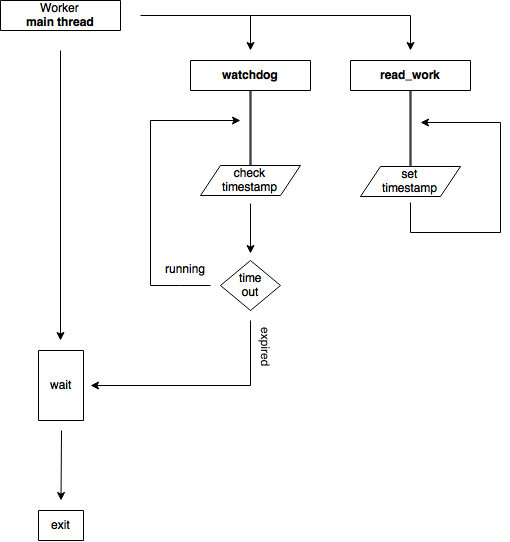
\includegraphics[width=\textwidth]{images/watchdog}
\caption{Schema della procedura di controllo sul tempo di esecuzione \label{fig: watchdog}}
\end{figure}
Il thread di \emph{watchdog}, letteralmente di sorveglianza, è adibito al controllo della \textbf{corretta esecuzione del worker}, in particolare al controllo che tale esecuzione, nell'occupare per eccessivo tempo le risorse del sistema, non vada a creare un collo di bottiglia che via via porta al collasso del programma. Per far questo esso viene eseguito in modalità \emph{detached} dal thread principale del worker ed è legato dalle operazioni che vengono eseguite dal processo da una serie di variabili: 
\begin{itemize}
	\item \textbf{\emph{pthread\_condition}}: condizione thread POSIX su cui è in attesa il thread principale del worker
	\item \textbf{\emph{flag}}: variabile legata alla condition di cui sopra che viene utilizzata per ciclare in attesa dello sblocco della condizione.
	\item \textbf{\emph{timestamp}}: valore temporale settato dal thread di lettura della richiesta / risposta in arrivo per confermare la lettura in corso di un pacchetto
\end{itemize}
Come appare da una prima analisi della struct del watchdog.
\begin{lstlisting}
typedef struct watchdog_thread {
  int status;                                     
  pthread_cond_t *worker_await_cond;             
  int *worker_await_flag;

  time_t killer_time;       // to schedule the watchdog wakeup
  time_t timeout_worker;    // to abort a thread run
  time_t timestamp_worker;  // timestamp last worker operation
} Watchdog, *WatchdogPtr;
\end{lstlisting}
Dove il \emph{killer\_time} ed il \emph{timeout\_worker} sono definiti dal file di configurazione per dare modo all'operatore di modellare l'implementazione sulle caratteristiche della macchina su cui gira il web switch. \\\\
Una più schematica rappresentazione del flusso di esecuzione è possibile vederla in figura \ref{fig: watchdog}.
In particolare quando vengono distaccati i thread ausiliari, il thread principale del worker si mette in attesa della fine di una delle condizioni di termine del servizio di cui si è già discusso sopra, fra cui anche lo scadere del massimo tempo di esecuzione disponibile. In particolare, ad ogni iterazione del thread di lettura, avremo un aggiornamento del timestamp del worker, per cui ogni volta che si ha l'arrivo di una risposta da reinoltrare o di una richiesta da soddisfare si assume il server come operativo od il client in ascolto. \\ 
Contemporaneamente il watchdog rimane in \emph{nanosleep} per un lasso di tempo pari a quello configurato, a meno dell'arrivo di segnali che vengono gestiti e dopo i quali il watchdog ritorna in attesa, scaduto il quale la variabile di timestamp viene controllata. Se risulta \emph{scaduta} viene aggiornato il flag di attesa del worker e gli viene segnalato di riattivarsi e di mettere in pratica le procedure di \emph{clean up} per scollegarsi dal client e dal server assegnato. \\\\
Osserviamo come questo controllo viene fatto su una variabile settata dal thread di lettura, permettendoci con semplicità di valutare eventuali problemi sia sulla linea fra web switch e macchina del cluster che fra web switch e client, evitando il pericoloso stato di attesa che porterebbe ad uno stallo del programma.

\newpage
\section{Politiche di scheduling}
 \label{sec: sched_p}
La schedulazione permette la selezione della macchina predisposta a rispondere alla richiesta HTTP appena arrivata da parte del client, si basa su una tecnica nota come \textbf{bilanciamento del carico}, ovvero la distribuzione del carico, solitamente di elaborazione o di erogazione di uno specifico servizio, tra più server. Questo permette di poter \textbf{scalare} sulla potenza di calcolo del cluster dietro al web switch, lasciando che siano diverse macchine a rispondere a seconda di quella che è più veloce, più performante, oppure monitorando costantemente lo stato dei server e scegliendo quello meno sottoposto ad una pressione del carico di lavoro. Le macchine, specificando hostname ed indirizzi IP, sono date in un apposito file di configurazione definito in \ref{ssec:config_server} .
\\
\\
Nella nostra implementazione \textbf{thread scheduler} si occupa di fornire,  ogni volta che viene invocato, una macchina selezionata secondo una delle due politiche che andremo ora a spiegare nel dettaglio.

\subsection{State-less: implementazione con Round-Robin}
L'algoritmo di scheduling Round-Robin (da adesso RR, \emph{n.d.r.}) è un algoritmo che agisce con prelazione distribuendo in maniera equa il lavoro, secondo una metrica stabilita in partenza. Vediamo quindi la struttura che si occupa di gestire la schedulazione tramite RR e che contiene i puntatori alle funzioni \emph{wrapper} che garantiscono il suo corretto funzionamento.\\
\begin{lstlisting}
typedef struct round_robin_struct {
  CircularPtr circular;

  ThrowablePtr (*weight)(CircularPtr circular, Server *servers, int server_num);
  ThrowablePtr (*reset)(RRobinPtr rrobin, ServerPoolPtr pool, int server_num);
  Server *(*get_server)(CircularPtr circular);
}RRobin, *RRobinPtr;

\end{lstlisting}
\begin{figure}[b]
\centering
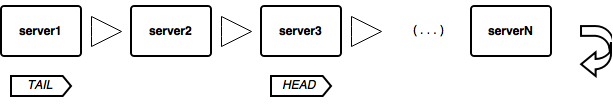
\includegraphics[width=\textwidth]{images/rrobin_stateless}
\caption{Schema di funzionamento del buffer circolare \label{fig: rrobin_sl}}
\end{figure}
Possiamo osservare come siano mantenuti i puntatori alle funzioni necessarie al caso di politica di scheduling \emph{state-aware}, ma per ora l'unica vera funziona a cui si farà riferimento è quella per il recupero del server correntemente selezionato. \\\\
L'algoritmo funziona utilizzando un \textbf{buffer circolare} come possiamo vedere in figura \ref{fig: rrobin_sl}: questo permette di iterare la selezione su una lista di elementi precedentemente caricata. Possiamo osservare che, oltre alle funzioni e le variabili necessarie a garantire l'accesso atomico all'area di memoria che contiene il buffer, necessario come vedremo nel caso \emph{state-aware} per evitare la concorrenza con il thread che si occupa dell'update dello stato, sono mantenuti:
	\begin{itemize}
  		\item Un puntatore all'array di server 
  		\item La posizione attuale del puntatore di \emph{testa} 
  		\item La lunghezza del buffer, necessaria anche per le operazioni di aggiornamento dei puntatori
  		\item I puntatori di \emph{testa} e \emph{coda} per avanzamento e lettura dal buffer
	\end{itemize}
	Le funzioni restanti permettono di inizializzare il buffer (oltre che di liberare con sicurezza l'area di memoria occupata) e di aggiornare i puntatori sopra menzionati.\\\\
\begin{lstlisting}
typedef struct circular_buffer {
  Server *buffer;
  int buffer_position;
  int buffer_len;
  
  Server *head;
  Server *tail;

  pthread_mutex_t mutex;

  ThrowablePtr (*allocate_buffer)(CircularPtr *circular, Server **servers, int len);
  ThrowablePtr (*acquire)(struct circular_buffer *circular);
  ThrowablePtr (*release)(struct circular_buffer *circular);
  void (*progress)(struct circular_buffer *circular);
  void (*destroy_buffer)(struct circular_buffer *circular);
} Circular, *CircularPtr;
\end{lstlisting}
È necessario quindi specificare tre passi per il corretto funzionamento, dopo aver dato un rapido sguardo alla struttura che lo rappresenta nella nostra implementazione. 
\\
\\
\textbf{Inizializzazione del buffer} in questa fase la struttura dati che rappresenta il buffer circolare, che abbiamo visto mantenere due puntatori di \emph{testa} e \emph{coda}, viene inizializzata associandovi un array di puntatori di strutture di tipo \emph{Server}, precedentemente allocata ed il cui pattern è stato fissato, e viene eseguita la funzione di allocazione del buffer: 
\begin{lstlisting}
/* inside allocate_buffer ... */
// allocating the buffer
circular->buffer = *servers;
circular->buffer_len = len;
// setting params
circular->head = circular->buffer;
circular->tail = circular->buffer + (len - 1);
\end{lstlisting}
In un'ottica di \emph{produttore vs consumatore}, chiaramente visibile nella figura precedente, è necessario che testa e coda non coincidano mai per evitare concorrenza. In questa implementazione si è deciso di separare l'accesso concorrente alla struttura, per il suo aggiornamento, e la lettura dei dati in essa contenuti. Quindi la \emph{testa} conterrà il puntatore al prossimo server da selezionare per schedulare la richiesta, mentre la \emph{coda} punterà all'area di memoria contenente il server attualmente selezione per la schedulazione. 
\\
\\
\textbf{Aggiornamento dei puntatori} per poter sfruttare le peculiarità di questa struttura dati è necessario che i due puntatori vengano aggiornati secondo l'aritmetica del buffer circolare per cui, una volta raggiunta l'estremità dell'array, il valore successivo della posizione corrente ritorna ad essere quello del primo valore dello stesso array. 
\\
Nel dettaglio viene eseguito, secondo le specifiche sopra riportate, nella nostra implementazione, la seguente funzione:
\begin{lstlisting}
void progress(CircularPtr circular) {
  // recomputing tail, head and buffer position
  circular->tail = circular->head;
  circular->buffer_position = (circular->buffer_position + 1) % circular->buffer_len;
  circular->head = circular->buffer + circular->buffer_position;
}
\end{lstlisting}
\textbf{Selezione del server} a questo punto, una volta che il thread chiamante invoca lo scheduler per recuperare il server che è stato selezionato dall'algoritmo, lo scheduler a sua volta invoca la funzione wrapper dalla struttura che gestisce la politica RR e questa esegue il codice ora riportato.
\begin{lstlisting}
/* inside get_server ... */
// allocating server ready struct
ServerPtr server_ready = malloc(sizeof(Server));

/* ... */

// stepping the circular buffer
circular->progress(circular),
// retrieving server from tail 
*server_ready = *(circular->tail);
return server_ready;
\end{lstlisting}
In conclusione quello che stiamo attuando è un \textbf{bilanciamento del carico uniforme} su ognuna delle macchine del cluster. Infatti, senza condizioni sullo stato delle macchine, iterando semplicemente sull'array dei server, ad ogni nuova connessione verrà assegnata una macchina diversa, alleggerendo tutti i server e pareggiando per ciascuno il carico. Il cluster manterrà il carico complessivo ma ogni singola unità contribuirà equamente a soddisfare le connessioni in arrivo.
\newpage
\subsection{State-aware: implementazione con monitor di carico}

\begin{figure}[t]
\centering
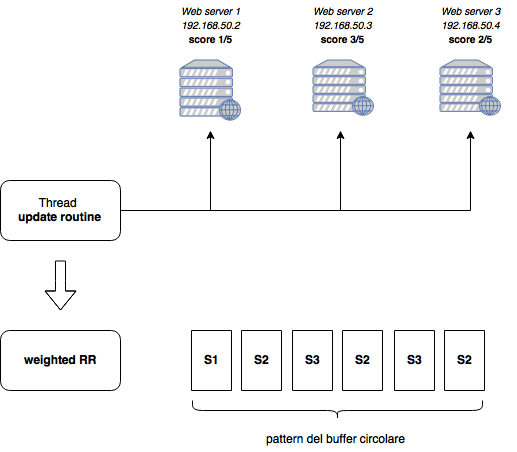
\includegraphics[width=\textwidth]{images/rrobin_stateaware}
\caption{Schema della procedura di aggiornamento dello stato dei server
\label{fig:rrobin_sa}}
\end{figure}
Un algoritmo di schedulazione cosiddetto \emph{state-aware} si occupa di selezionare la macchina a cui inoltrare la connessione basandosi non solo sulla conoscenza delle macchine presenti nel cluster ma anche sul loro status. In particolare, in questa implementazione, si è deciso di ricorrere all'analisi dei risultati di un \textbf{monitor di carico} presente su ciascuna delle macchine del cluster (in riferimento alle assunzioni progettuali, questi è i modulo \emph{ApacheStatus} di cui si parlerà più avanti in \ref{sssec:apachestatus}). Tale monitor, che ritorna una serie di parametri indici dell'attuale impiego di risorse della macchina, permette di definire un \textbf{algoritmo pesato} per la selezione del server che risponderà alla connessione in arrivo al web switch. \\
Anche in questo caso andremo a determinare una serie di passi che vengono seguiti, tenendo conto che in fase progettuale \emph{si è deciso di sfruttare lo stesso algoritmo RR} già utilizzato nel caso \emph{state-less}, ma che ricordiamo essere stato predisposto per una ulteriore versione pesata. Per far questo si lavora sulla struttura Server \\\\
\textbf{Detachment del thread di update} nei file di configurazione dell'applicazione è possibile definire due livelli di lavoro:
	\begin{itemize}
		\item \textbf{AWARENESS\_LEVEL\_LOW} che corrisponde ad una versione state-less dell'algoritmo RR e si riporta al caso precedente
		\item \textbf{AWARENESS\_LEVEL\_HIGH} che corrisponde all'algoritmo state-aware e che necessiterà di una routine di aggiornamento dello stato delle macchine del cluster
	\end{itemize}
	Il secondo caso è proprio quello qui descritto e corrisponde a lavorare utilizzando, oltre al thread principale che si occupa di accettare le connessioni in arrivo, un \textbf{thread predisposto alla sola verifica dello stato dei server}. Tale thread viene istanziato nel momento in cui viene inizializzato lo scheduler e vengono allocate le strutture dati alla base di RR. \\
	Il lavoro di tale thread, che ora vedremo nel dettaglio, è quello deducibile da figura \ref{fig:rrobin_sa}.\\\\
\textbf{Routine di score} all'interno di questa routine, che viene eseguita da un thread distaccato e che viene eseguita una volta ogni \emph{up\_time} secondi, tempo di update in secondi definito dall'utente nei file di configurazione, viene richiamata più volte la funzione che si occupa di recuperare e parsare l'interrogazione del modulo \emph{ApacheStatus} e recupare da questa i \textbf{worker in \emph{idle state} ed i worker in \emph{busy state}}. A questo punto si va a modificare il nodo della pool dei server precedentemente allocata (di cui si è già parlato in \ref{ssec: sched}). Viene quindi eseguita la sequente routine. \\
\begin{lstlisting}
/* inside apache_score ... */
// retrieving status from remote Apache machine
throwable = apache_status->retrieve(apache_status);   
//checking for errors or if server is currently down
if (throwable->is_an_error(throwable)) {
  server->weight = WEIGHT_DEFAULT;
  server->status = SERVER_STATUS_BROKEN;
  return throwable->thrown(throwable, "apache_score");
} else {
  server->status = SERVER_STATUS_READY;
}

/* ... */
int score;
int IDLE_WORKERS  = apache_status->idle_workers;
int TOTAL_WORKERS = apache_status->busy_workers + IDLE_WORKERS;

// calculating and setting score - mapping in [w, W]
score = (IDLE_WORKERS   - WEIGHT_DEFAULT)   *
        (WEIGHT_MAXIMUM - WEIGHT_DEFAULT)   /
        (TOTAL_WORKERS  - WEIGHT_DEFAULT)   +   WEIGHT_DEFAULT;
server->weight = score;
\end{lstlisting}
Alla fine quello che ottengo è uno \textbf{score} che vado a settare nel nodo contenuto nella \textbf{pool dei server} che viene definito dalla relazione matematica che è così esplicitata:
\begin{align*}
  score\Big(\frac{IDLE\_WORKERS}{TOTAL\_WORKERS}\Big) ~ \in ~ [w, W]
\end{align*}
ottenendo quello che un \emph{mapping} del rapporto fra i worker occupati nella macchina ed i worker totali a disposizione di Apache per rispondere ad una richiesta in arriva. Tale indice viene memorizzato come \emph{peso del server nel cluster}.\\
Notiamo che nel caso ci siano problemi nel recuperare l'indice di score si supporrà che il server non è momentaneamente disponibile ed il suo status verrà segnalato come BROKEN, fino al prossimo aggiornamento.\\\\
\textbf{RR pesato} dai nodi della pool dei server aggiornati con il loro peso viene costruito, secondo lo schema in figura \ref{fig:rrobin_sa}, un pattern dei server secondo il loro peso, di modo da distribuire il carico secondo sempre un algoritmo RR, ma in cui per ogni sequenza il server viene selezionato un numero di volte pari al suo peso. Dunque una macchina comparirà massimo \emph{W} volte in caso di basso carico di lavoro ed al minimo \emph{w} volte in condizioni di forte stress. I due parametri sono, in questa implementazione, macro che possono essere modificate a seconda dei limiti delle macchine del proprio cluster, di default \emph{w = 1} e \emph{W = 5}, soggetti al tuning del web switch in fase di installazione ed ottimizzazione. Alla prima iterazione tutte le macchine sono di default settate con peso minimo (pari a \emph{w})\\\\
In conclusione, con questa opzione abilitata, si ha la possibilità di ridistribuire equamente il lavoro, permettendo ah Heimdall di adattare la distribuzione del carico a secondo dello stato attuale, evitando di sovraccaricare nodi sensibili allo stress in determinate condizioni o che sono stati sottoposti già ad uno stress eccessivo. Si è scelto di riadattare RR per ottenere una soluzione modulare e che fosse facile riadattare ed ottimizzare a seconda di entrambe le condizioni operative, sia senza che con conoscenza dello stato delle macchine. Osserviamo infatti che in entrambi i casi RR risulta pesato, nel secondo caso preso in esame tale peso non è più fisso e minimo ma variabile dipendentemente dalle condizioni delle macchine.\\\\
La ricerca di una soluzione modulare che possa essere presa poi in esame da futuri sviluppatore e possa essere oggetto di un \emph{tuning} più approfondito, è stata intrapresa perseguendo il principio per cui \emph{simplicity favours regularity}.

\subsubsection{Modulo Apache Status}
\label{sssec:apachestatus}
Il modulo Apache Status (mod\_status)\cite{mod_status} è un modulo che fornisce informazioni sull'attività e le prestazioni del server in cui è installato. Questo modulo è disponibile nella versione base di Apache senza il bisogno di dover scaricare nessun altro componente aggiuntivo. Per utilizzarlo è necessario solo attivarlo nella configurazione del web server. Il modulo formatta in una pagina HTML tutta una serie di statistiche e dati facilmente leggibili da un essere umano (oppure nella sua variante machine readable, versione utilizzata in questa applicazione).
\\
I dettagli che fornisce sono:

\begin{itemize}
  \item Il numero di worker che servono le richieste;
  \item Il numero totale di worker in pausa;
  \item Lo stato di ciascun worker: il numero di richieste che il worker ha eseguito e il numero totale di bytes serviti;
  \item Il tempo da quando il server è stato avviato/riavviato;
  \item Il numero medio di richieste per secondo, il numero di bytes serviti per secondo e il numero medio di bytes per richiesta.
\end{itemize}

Quindi, tramite questo modulo, Heimdall è in grado di verificare lo stato di ciascuna macchina (con a bordo un server Apache), senza la necessità di installare alcun componente aggiuntivo o di valutare empiricamente il carico del server tramite, per esempio, il tempo di risposta di quest'ultimo.

\subsubsection{Performance della politica state aware}
È interessante osservare l'effettivo lavoro dello scheduler e della politica di \emph{state awareness} già commentata, in una condizione di forte stress delle macchine, nell'estratto del file di log che segue. La situazione proposta è stata ottenuta sovraccaricando una delle macchina del cluster e lasciando che il web switch si accorgesse di tale sovraccarico per bilanciare le richieste in arrivo.

\begin{lstlisting}[basicstyle=\fontsize{6.4}{7}\selectfont\ttfamily]
[Wed Feb 10 11:31:44 2016] - 192.168.1.3 to: 192.168.1.4 - worker: 3032 - GET / HTTP/1.1
[Wed Feb 10 11:31:44 2016] - 192.168.1.3 to: 192.168.1.5 - worker: 3031 - GET / HTTP/1.1
[Wed Feb 10 11:31:45 2016] - 192.168.1.3 to: 192.168.1.6 - worker: 3040 - GET / HTTP/1.1
[Wed Feb 10 11:31:45 2016] - 192.168.1.3 to: 192.168.1.5 - worker: 3039 - GET / HTTP/1.1
[Wed Feb 10 11:31:45 2016] - 192.168.1.3 to: 192.168.1.6 - worker: 3038 - GET / HTTP/1.1
[Wed Feb 10 11:31:45 2016] - 192.168.1.3 to: 192.168.1.5 - worker: 3037 - GET / HTTP/1.1
[Wed Feb 10 11:31:45 2016] - 192.168.1.3 to: 192.168.1.6 - worker: 3036 - GET / HTTP/1.1
[Wed Feb 10 11:31:45 2016] - 192.168.1.3 to: 192.168.1.5 - worker: 3035 - GET / HTTP/1.1
[Wed Feb 10 11:31:45 2016] - 192.168.1.3 to: 192.168.1.6 - worker: 3034 - GET / HTTP/1.1
\end{lstlisting}
\begin{figure}[H]
\centering
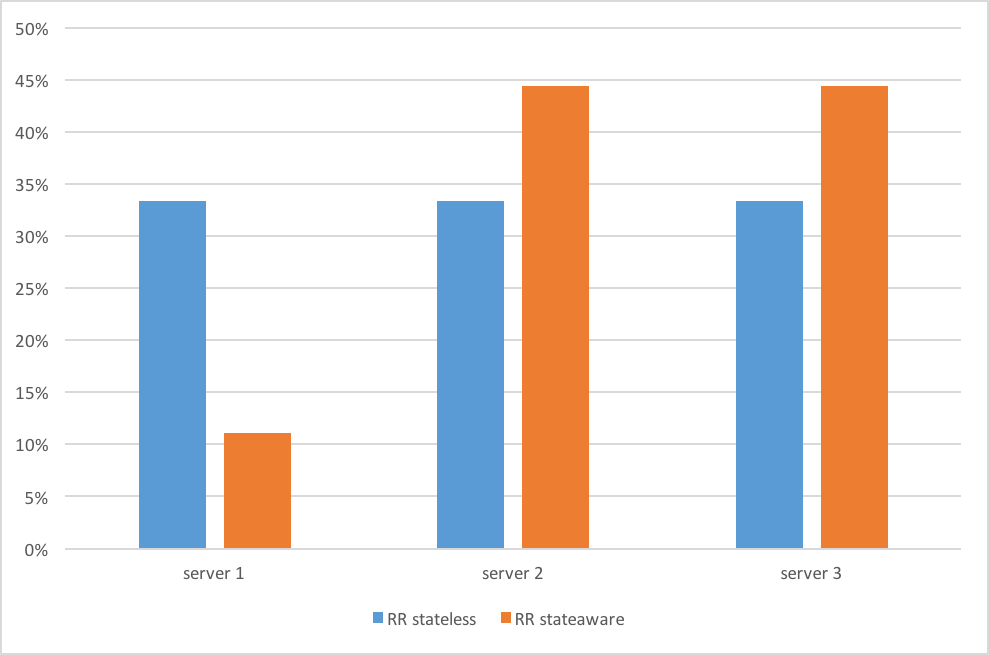
\includegraphics[width=\textwidth]{images/round_robin_cfr}
\caption{Ripartizione del carico di lavoro, \emph{confronto fra politica state-less e state-aware}\label{fig: rrobin_cfr}}
\end{figure}
In queste circostanze, considerato che secondo la nostra implementazione un server deve apparire almeno una volta nel buffer circolare, considerato che uno dei server era stato sottoposto a forte carico e che gli altri due server avevano un peso relativo superiore di tre unità, otteniamo che il server a venire meno sottoposto a connessioni in arrivo è proprio il server il cui carico di lavoro è già calcolato come particolarmente elevato. \\
È possibile accertarlo sia dall'estratto del file di log riportato che dalla figura \ref{fig: rrobin_cfr} che ne quantifica i risultati.
\newpage
\section{Performance}
Abbiamo visto più volte durante questa trattazione che è stato necessario sottoporre a \emph{tuning} l'effettiva implementazione del server o che si consiglia di modellare quanti più aspetti possibili del web switch secondo la rete e le capacità della macchina. Riportiamo qui alcuni test che sono stati utilizzati in fase di progettazione per modellare la risposta del programma. I test sono stati condotti su:
  \begin{itemize}
    \item Macchina virtuale con Ubuntu Server 14.04 - 512 MB di RAM 
    \item Macchina con Ubuntu Desktop 15.10 - 6 GB di RAM, processore Intel i3 (1,9 GHz)   
  \end{itemize}
Nel primo caso durante tutta la fase di sviluppo, nel secondo caso durante i test di carico per dare possibilità al web switch di non dover dipendere dall'hardware virtualizzato. Consideremo in tutti i casi la rete non saturata, in particolare non consideriamo la possibilità di influenze da parte di traffico generato da altre fonti essendo i test, per necessità, condotti o con una rete locale fra macchine collegate da uno switch di rete, oppure in locale su diverse macchine virtuali. 
\\
\\ 
\textbf{Numero di processi e limite dei file descriptor} durante i test che seguono il numero di worker, variabile nelle configurazioni, è fissato a 10 come di default. Questo è stato giustificato da un'osservazione in fase sperimentale: non esiste una vera e propria variazione apprezzabile delle performance all'aumentare del numero di worker sopra i 10-15. Il valore di 10 unità è stato proposto per evitare sia un eccessivo utilizzo della memoria, sia per limitare il lavoro complessivo durante la creazione dei thread, sia per evitare ulteriore \emph{overhead} dovuto al cambio di contesto. 
\\
Inoltre il numero di file descriptor utilizzabili per l'apertura delle socket è fissato, come da default nei file di configurazione, a 4096.
\\
\\
\textbf{Numero di connessioni e di richieste} per poter simulare l'approccio più "aggressivo" di un browser moderno, si è pensato di testare il programma permettendo a \emph{httperf} di inviare 10 richieste per ogni connessione instaurata. Quindi ogni worker avrà una coda di 10 richieste da smaltire.
 
\subsection{Test di carico}
Il \textbf{confronto dei tempi di risposta} è stato condotto unendo ad uno switch di rete tre macchine, una su cui girava il web switch sull'ambiente desktop di cui sopra, una da cui veniva condotti i \emph{benchmark} sia via browser che sia attraverso il tool da linea di comando \emph{httperf} di cui parleremo nell'appendice \ref{ssec: httperf}. \\\\
Mantenendo \emph{frequenza di richieste per secondo} costante, osserviamo due situazioni diverse, riscontrate con l'aumentare di tale frequenza. In figura \ref{fig: cfr_reply_time1} possiamo vedere come ci sia un valore intorno al quale è possibile registrare oscillazioni, di decimi di millesimi di secondo, dovute probabilmente allo stato della macchina ospitante il web switch. Tuttavia è significativo come all'aumentare del rate (per esempio a \emph{50 req/s}) cominciamo ad osservare un nuovo livellamento di dei tempi di risposta, maggiormente significativo. Questo a causa del carico di lavoro che comincia a giungere alla macchina e che porta ad una situazione stabile di occupazione dei worker. \\ 
Questa osservazione è suffragata dall'analisi del grafico in figura \ref{fig: cfr_reply_time2}. dove possiamo vedere come, con una frequenza di 100 req/s, si ha un aumento ripido dei tempi di risposta, dovuto al fatto che vengono fatte sempre più richieste, con un tempo almeno doppio di quanto occorre al web switch per liberare i propri worker per poter rispondere alle nuove connessioni. Andremo ora a vedere più nel dettaglio, nello \emph{stress test}, questa peculiarità del nostro programma.
\begin{figure}[H]
\centering
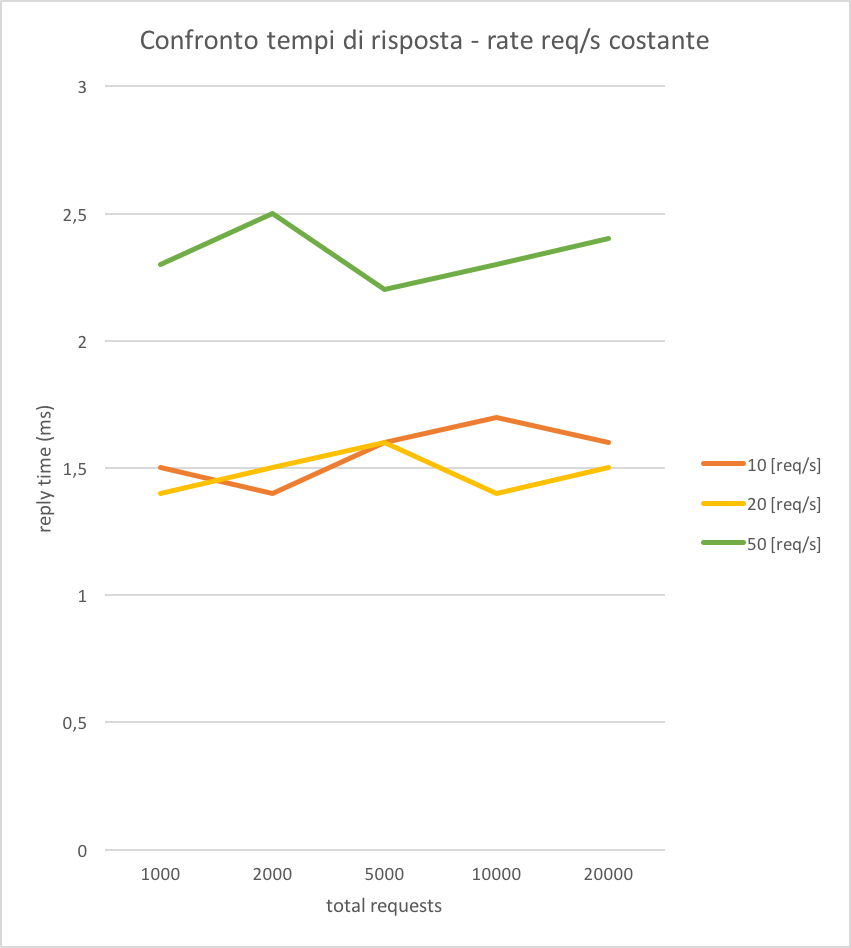
\includegraphics[width=\textwidth]{images/cfr_reply_time1}
\caption{Confronto fra i tempi di risposta con diversi rate all'aumentare delle richieste. Si osserva lo stabilizzarsi intorno ad un livello medio.\label{fig: cfr_reply_time1}}
\end{figure}\begin{figure}[H]
\centering
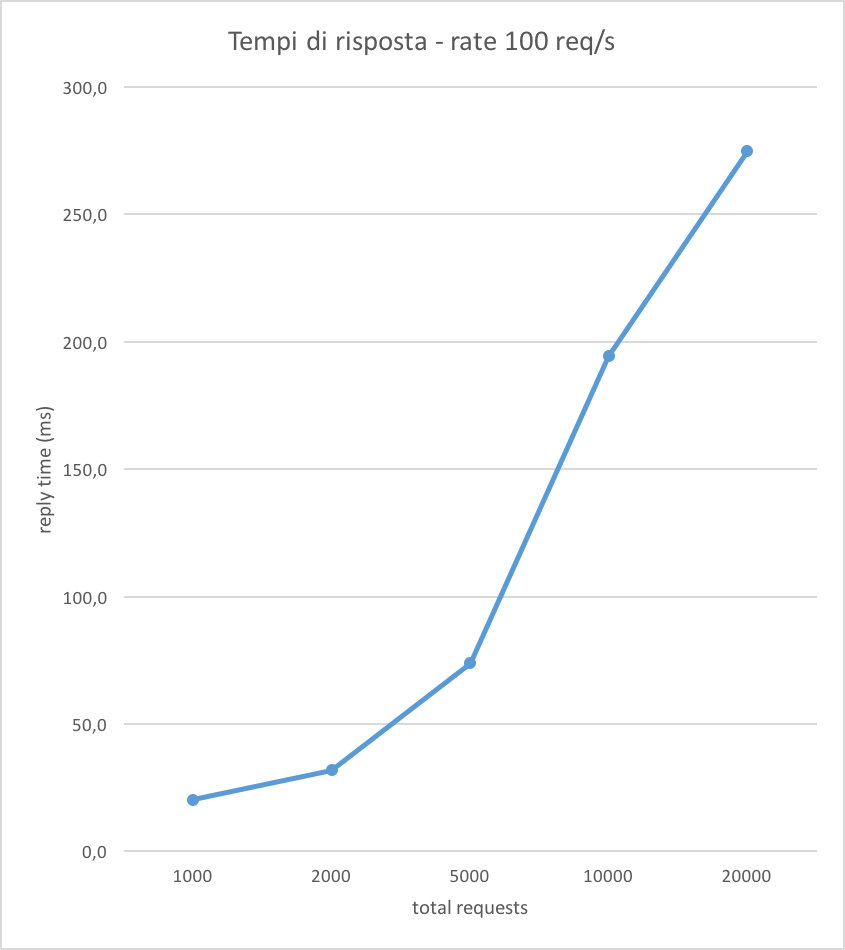
\includegraphics[width=\textwidth]{images/cfr_reply_time2}
\caption{Crescita dei tempi di risposta all'aumentare del numero di richiesta, si osserva come il lavoro dei worker non è sufficiente è compensare la frequenza delle richieste. \label{fig: cfr_reply_time2}}
\end{figure}
\subsection{Valutazione delle performance}
In questo caso abbiamo deciso di testare il programma in un possibile scenario applicativo vicino a quello di uno sviluppatore indipendente o di uno studente. Valutando le dimensioni tipiche di un \emph{Virtual Private Server} di fascia \emph{entry level}, abbiamo utilizzato una macchina virtuale con 512 MB di RAM con sistema operativo Ubuntu Server. Le condizioni del test includevano un numero di richieste fisso pari a 10000 richieste in arrivo, facendo variare la frequenza con cui queste giungevano. Si è deciso di prendere in considerazione sia il tempo di risposta che la frequenza con cui queste risposte giungevano al client che generava il carico di lavoro. \\\\ 
Quello che si è potuto constatare, relativamente alla figura \ref{fig: repvsfreq}, è il crescere dei tempi di risposta linearmente, con un andamento paragonabile a quello osservato ma in questo caso riconducibile ad un carico di richieste al secondo, piuttosto che all'aumentare delle connessioni. È significativo osservare la diminuzione della pendenza per alte frequenze di richieste, riconducibile al raggiungimento della saturazione delle risorse del web switch che lavora ora ad un regime massimo.\\\\
Sempre dallo stesso grafico, analogamente, è possibile osservare come, ad un aumento dei tempi di risposta corrisponde, all'aumentare della frequenza di invio delle richieste, un aumento della frequenza di ricezione delle risposte fino un livello di assestamento. Difatti si ha, mantenendo le connessioni costanti, il raggiungimento di un livello medio attorno al quale rimane, a meno di oscillazioni, una apprezzabile frequenza di risposta. Si può dedurre l'esistenza di un livello di saturazione che non può essere ne abbattuto, a causa della frequenza elevata, ne innalzato a causa della frequenza fissa con il quale i worker si liberano e vengono rioccupati da nuove connessioni. Tale frequenza di lavoro è dovuta sia alla presenza di una coda delle richieste che garantisce una certa inerzia, sia al raggiunto limite delle capacità della macchina di operare il context switching e nel ricreare i thread.. Il che ci porta a concludere che a pieno regime il web switch riesce ad adeguarsi alla velocità con cui sono in arrivo le richieste e soddisfare la domanda, seppure con un ritardo lineare nei tempi di risposta.
\begin{figure}[H]
\centering
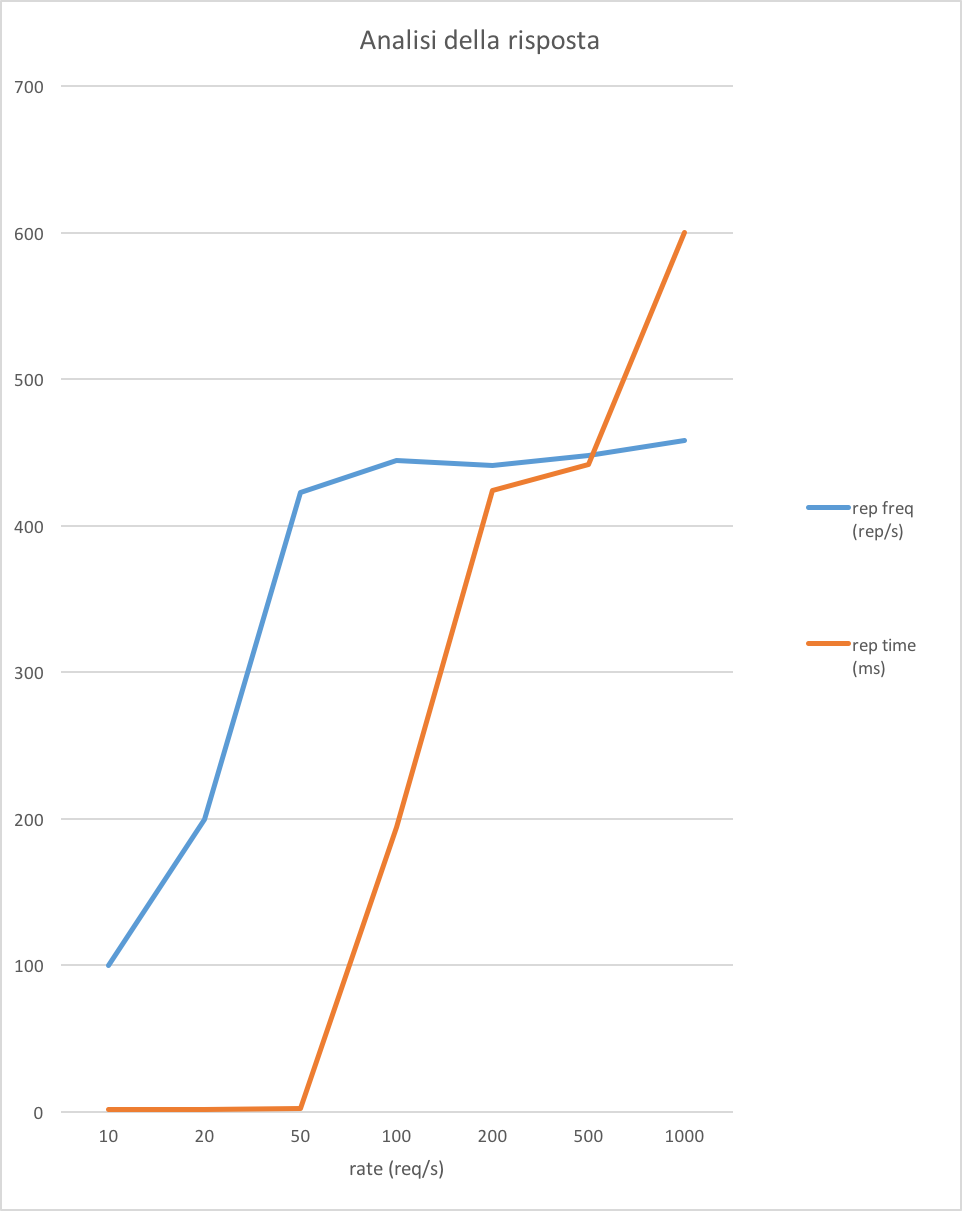
\includegraphics[width=\textwidth]{images/repvsfreq}
\caption{Analisi delle performance confrontando i tempi di risposta e la frequenza con cui la risposta viene fornita.\label{fig: repvsfreq}}
\end{figure}\subsection{Comparazione con Apache}
Con le caratteristiche della macchina di test già riportate nella sezione precedente, si è proceduto a verificare, una volta valutate le performance a regime, quale fosse l'overhead aggiunto dal nostro programma ad una delle macchine del cluster montante un web server Apache. \\
Possiamo verificare le statistiche di questo test con il grafico di figura \ref{fig: apachevsheimdall}. Si osserva come, malgrado i tempi di risposta siano inferiori, tale differenza diventa poco apprezzabile nel momento in cui si ha una maggiore frequenza nelle risposte da parte del web server Apache. In conclusione si osserva come la durata del test è, in entrambi i casi, irrisoria e confrontabile. Per cui l'overhead aggiunto, per quanto non possa essere eccessivamente abbattuto, risulta essere accettabile per un'applicazione effettiva del web switch.
\begin{figure}[H]
\centering
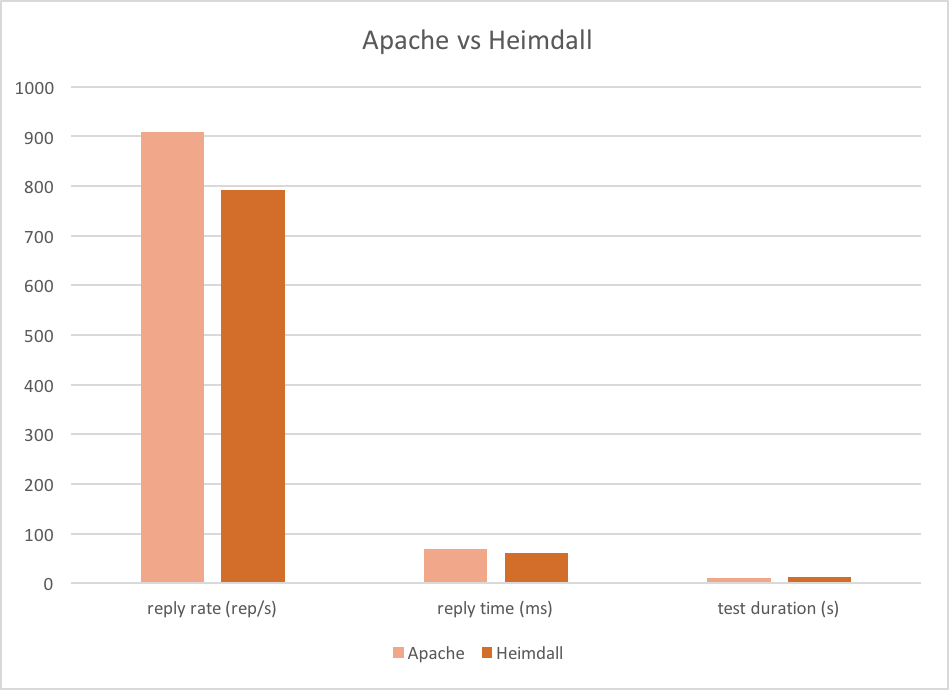
\includegraphics[width=\textwidth]{images/apachevsheimdall}
\caption{Confronto dei tempi di risposta di un web server Apache con il web switch Heimdall(10000 richieste per una frequenza di 100 req/s).\label{fig: apachevsheimdall}}
\end{figure}
\subsection{Limitazioni}
Durante i test che sono appena stati descritti, in particolare quelli con macchina virtuale, monitorando anche le risorse della macchina, si è potuto constatare che era presente un'\textbf{occupazione della RAM} crescente e, in alcuni casi, eccessiva, al punto da non permettere alla macchina di proseguire ulteriormente nelle operazioni. Tale occorrenza, per quanto rara e verificabile solamente nel caso di un carico veramente elevato, è dovuta alla non corretta liberazione della memoria nei processi che agiscono da worker: un'analisi più accurata ha portato alla luce la presenza di una grande quantità di memoria virtuale allocata e liberata correttamente ma, con una frequenza elevata di richieste in arrivo, non viene liberata memoria con la stessa velocità con cui viene occupata, portando ad una situazione pericolosa di saturazione. \\
Ben altra saturazione è stata evitata, invece, limitando il \textbf{numero di file descriptor} associabili ad una socket, imponendo alla macchina di rispettare un certo limite ed evitando, quindi, di portare il programma al blocco nel caso di termine delle risorse a disposizione del processo. \\\\
È possibile apprezzare in figura \ref{fig: fd_memory} l'occupazione di memoria e di file descriptor durante uno \emph{stress test} poco prima del raggiungimento del limite di memoria a disposizione. 
\begin{figure}[H]
\centering
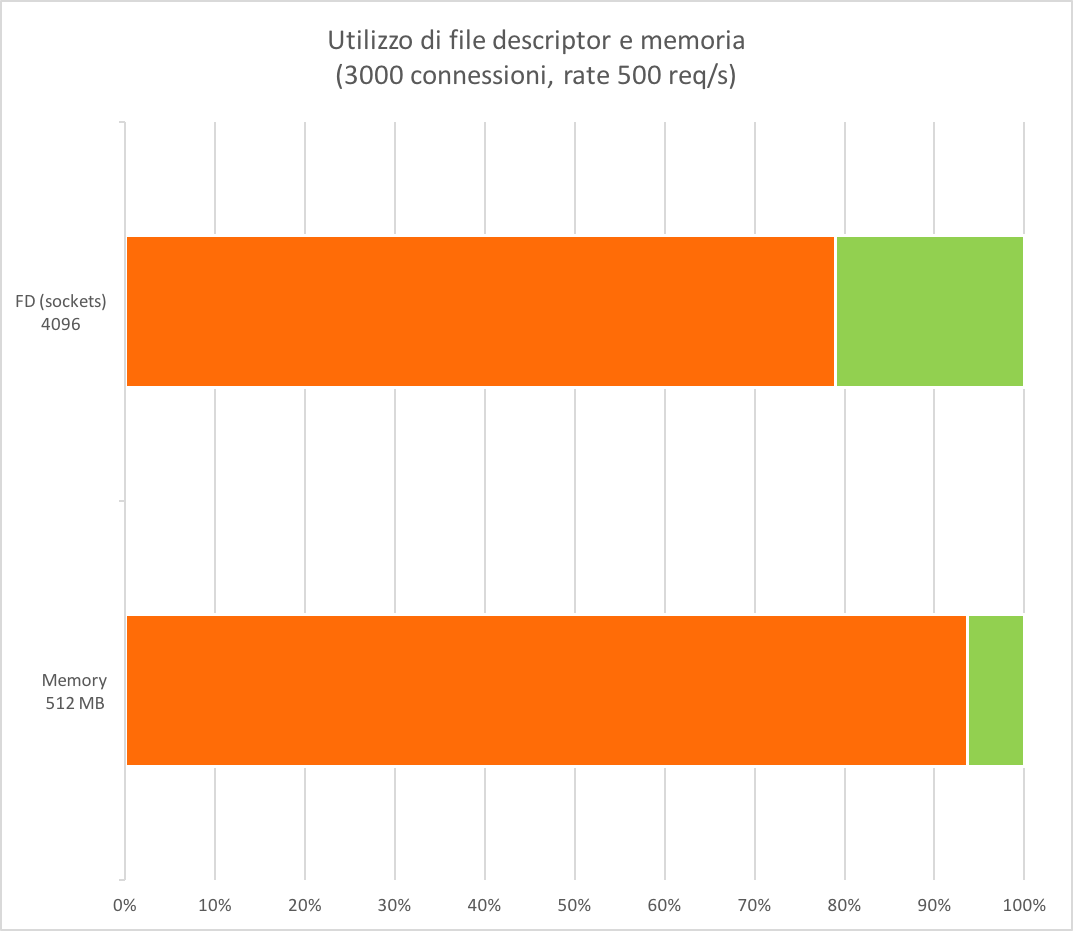
\includegraphics[width=\textwidth]{images/fd_memory}
\caption{Visualizzazione dell'occupazione di memoria e fd durante uno stress test.\label{fig: fd_memory}}
\end{figure}
\subsection{Conclusioni}
\newpage
\section{Future implementazioni}
In questo capitolo vogliamo parlare di alcune ulteriori proposte che ci sono venute in mente per poter migliorare Heimdall. Si tratta quindi di sviluppi futuri che abbiamo elaborato nel corso dello sviluppo del progetto e a seguito di alcune limitazioni che abbiamo identificato nei componenti da noi sviluppati.
\subsection{Analisi della richiesta}
Come abbiamo già visto nei paragrafi dedicati al \emph{parsing} delle richieste e delle risposte HTTP, è stato possibile, in fase progettuale, scegliere su quali \emph{header} basare il funzionamento elementare del web switch. Abbiamo visto anche come i file di configurazione garantiscono veramente molta flessibilità al sistemista in sede di installazione.
\\
Non è difficile immaginare che, in una futura implementazione, l'applicazione non possa basarsi su file di configurazione più dettagliati e quindi possibilità di utilizzare tutti i parametri a disposizione per l'analisi di richiesta e risposta. Per cui si aprono scenari in cui si possono, ad esempio, configurare server di \emph{cache di immagini} in particolari posizioni del cluster, oppure utilizzare un algoritmo di schedulazione \emph{state-aware} che si basi anche sulla grandezza dei file richiesti e che quindi, a monte, eviti il carico di macchine sensibili.
\subsection{Webserver performante}

\newpage
\section{Ulteriori proposte}

\subsection{Worker come thread}
Abbiamo visto nel paragrafo dedicato che il Worker nel contesto attuale è un processo figlio del processo principale. Questa è stata una scelta progettuale dettata da alcune caratteristiche che ritenevamo opportune per il WebSwitch, ad esempio l'isolamento della connessione HTTP. Infatti nella nostra architettura ogni Worker lavora in un contesto indipendente dagli altri quindi un eventuale problema con una connessione non danneggia le altre. L'utilizzo però di processi ci ha portato a dover gestire alcuni piccoli problemi, infatti ci siamo resi conto degli "elevati" tempi di fork() e anche dei tempi che occorrono ad eseguire un cambio di contesto. Inoltre ci siamo dovuti equipaggiare di memoria condivisa per poter scambiare dati con i Worker e adottare un meccanismo di messaggi per l'invio di file descriptor. Pensiamo quindi che utilizzare un approccio a Thread ci permetta di essere più performanti in quanto si sa che la creazione e la schedulazione di un thread è più veloce rispetto a quella di un processo, inoltre come sappiamo i thread condividono lo stesso spazio di memoria e questo evita i problemi di memoria condivisa e invio file descriptor.

% \subsection{Pool Manager come processo}

% --- References ---  
%
% bibtex is used to generate the bibliography. The babplain style
% will generate numeric references (e.g. [1]) appropriate for theoretical
% computer science. If you need alphanumeric references (e.g [Tur90]), use
%
% \bibliographystyle{babalpha-lf}
%
% instead.


\newpage
%\bibliographystyle{babplain-lf}
%\bibliography{references}
\renewcommand{\refname}{\normalfont\selectfont\normalsize\textbf{Annotazioni}} 
\begin{thebibliography}{9}
\bibitem{apache_server}
  Apache HTTP Server Project, \url{https://httpd.apache.org/}
\bibitem{throwable_java}
  Throwable (Java Platform SE 8), \url{https://docs.oracle.com/javase/8/docs/api/java/lang/Throwable.html}
\bibitem{http_1.1}
  RFC: 2616: Hypertext Transfer Protocol - HTTP/1.1, \url{https://tools.ietf.org/html/rfc2616}
\bibitem{persistent_connections}
  RFC: 2616: Persistent Connections, \url{https://tools.ietf.org/html/rfc2616#section-8.1}
\bibitem{pipeling}
  RFC: 2616: Pipeling, \url{https://tools.ietf.org/html/rfc2616#section-8.1.2.2}7
\bibitem{full_duplex}
  RFC: 793: Connection Establishment and Clearing, \url{https://tools.ietf.org/html/rfc793#section-2.7}
\bibitem{mod_status}
  Apache Module: mod\_status, \url{http://httpd.apache.org/docs/2.2/mod/mod_status.html}
\bibitem{cmake} 
  CMake \url{http://cmake.org}
\bibitem{vagrant}
  Vagrant by HashiCorp \url{http://www.vagrantup.com}
\bibitem{virtualbox}
  Oracle VM VirtualBox \url{http://www.virtualbox.com}
\bibitem{gdb}
  GDB: The GNU Project Debugger, \url{https://www.gnu.org/software/gdb/}
\bibitem{htop}
  htop: an interactive process viewer for Unix, \url{http://hisham.hm/htop/}
\bibitem{valgrind}
  Valgrind, \url{http://valgrind.org/}
\bibitem{httperf}
  Httperf by HP Labs \url{http://www.labs.hpe.com/research/linux/httperf}
\bibitem{postman}
  Postman Chrome Extension \url{http://www.getpostman.com}
\bibitem{apple}
  Apple Safari \url{http://www.apple.com/safari}
\bibitem{chrome}
  Google Chrome Web Browser \url{http://www.google.com/chrome}
\bibitem{firefox}
  Mozilla Firefox Web Browser \url{http://www.mozilla.org/it/firefox}
\end{thebibliography}

% --- Appendices --- 
\newpage
\appendix
\newpage
\section{Manuale per l'uso}
L'installazione e l'utilizzo del web switch Heimdall sono progettati per essere il più immediati possibile. Vediamo nel dettaglio quale è la procedura per installare e compilare per la prima volta l'intero progetto. 
\\
\\
\textbf{Nota:} nel caso in cui si voglia procedere direttamente all'esecuzione del programma, il cui file binario è allegato a questa relazione, è necessario procedere dalla \ref{ssec: configuration} per modificare alcuni file di configurazione e creare alcune cartelle necessarie all'esecuzione.
\subsection{Download}
Il progetto può essere recuperato dalla repository pubblica ospitata su GitHub all'indirizzo:
\\
\url{https://github.com/HeimdallProject} 
\\
La repository scaricata conterrà:
\begin{itemize}
  \item codice sorgente;
  \item script di installazione e compilazione;
  \item file necessari alla compilazione del progetto.
\end{itemize}
\subsection{Dipendenze}
È incluso il \emph{binary} del progetto all'interno del file allegato alla relazione, tuttavia in caso di download del progetto dalla repository su GitHub, per procedere alla compilazione che vedremo al punto successivo, è necessario installare \emph{CMake}.\\
CMake\cite{cmake} è una famiglia di tool \textbf{open-source} e \textbf{cross-platform}, disegnati per poter controllare il processo di compilazione attraverso una piattaforma indipendente sia dall'architettura che dall'ambiente di compilazione prescelto sulla propria macchina. Tale obiettivo viene raggiunto tramite un file di configurazione che possiamo trovare nella cartella del progetto sotto il nome \emph{CMakeLists.txt}. Nel nostro caso è stato utilizzato per poter far fronte, utilizzando un tool professionale, al grande numero di dipendenze e poter gestire sia la ricerca di \textbf{package e librerie} particolari sia l'utilizzo di particolari \textbf{direttive di precompilazione}, il tutto mantenendo un file di configurazione compatto e facilmente leggibile. \\\\
La versione di minima di CMake necessaria è la 3.2 e può essere scaricata sia dal sito sopra indicato che, procedendo da linea di comando. Vediamo brevemente come fare, tenendo conto che, per l'installazione di software, è necessario possedere i privilegi dell'utente \emph{root}.
\begin{lstlisting}
$ sudo apt-get install software-properties-common
$ sudo add-apt-repository ppa:george-edison55/cmake-3.x
$ sudo apt-get update
$ sudo apt-get install cmake
\end{lstlisting}
Altrimenti si può procedere alla compilazione di cmake stesso. Anche in questo caso è necessario disporre dei privilegi di \emph{root} (cambiare il numero della versione per scaricare la versione desiderata).
\begin{lstlisting}
$ sudo apt-get install build-essential
$ wget http://www.cmake.org/files/v3.2/cmake-3.2.2.tar.gz
$ tar xf cmake-3.2.2.tar.gz
$ cd cmake-3.2.2
$ ./configure
$ make
$ sudo make install
\end{lstlisting}
\subsection{Compilazione}
Una volta installato il programma utilizzato per la compilazione del progetto, si può procedere alla fase finale di preparazione per l'esecuzione del programma eseguendo lo script \textbf{install.sh} presente all'interno della cartella di installazione.
\begin{lstlisting}
$ cd <installation folder>
$ sh install.sh 
\end{lstlisting}
A questo punto si può procedere direttamente al passo di esecuzione illustrato in \ref{ssec: execution}.
\\
\\
In alternativa è possibile procedere alla sola compilazione del progetto, con il suggerimento di creare una cartella separata in cui salvare i file relativi alla compilazione.
\begin{lstlisting}
$ cd <installation folder>
$ mkdir build
$ cd build
$ cmake ..
$ make WebSwitch
\end{lstlisting}
\subsection{Modifica file di configurazione} \label{ssec: configuration}
Nel caso si disponesse già di una copia dei file binary o si avesse compilato il programma indipendentemente dallo script illustrato al punto precedente, è possibile procedere alla configurazione delle cartelle necessarie all'esecuzione del programma eseguendo lo script \textbf{config.sh} fornito.
\begin{lstlisting}
$ cd <installation folder>
$ sh config.sh 
\end{lstlisting}
Per ulteriori necessità e in particolare per il tuning del web switch, si può fare riferimento ai file presenti nell cartella \emph{<installation folder>/code/config}. 
\\
Qualora si volessero modificare la posizione delle cartelle contenenti i file di log e le socket, necessari all'esecuzione del programma, è possibile modificare, all'interno di \emph{code/config/heimdall\_config.conf} le linee seguenti:
\begin{lstlisting}
# File for request logging
log_file_req <absolute req log path>/heimdall_req.log

# File for response logging
log_file_resp <absolute resp log path>/heimdall_resp.log

# Unix sockets path
sockets_path <absolute socket path>/sockets/  
\end{lstlisting}
Per modificare la \textbf{configurazione del cluster}, si possono specificare le diverse macchine all'interno del file \emph{code/config/server\_config.conf}, scrivendo per ognuna indirizzo ip ed il nome del server.
\\
\subsection{Esecuzione} \label{ssec: execution}
A questo punto si può supporre creata una cartella \emph{build} dov'è presente il file binario del progetto. Supponendo di aver configurato il nostro web switch adeguatamente, possiamo procedere ad avviare l'applicazione da linea di comando.
\begin{lstlisting}
$ cd build
$ ./WebSwitch  

\end{lstlisting}
Nota che il web switch è di default configurato per essere in ascolto sulla porta 8080. Per metterlo in ascolto sulla porta 80 è necessario possedere i privilegi di root.
\\
\\
Buon lavoro!
\newpage
\section{Vagrant}
Durante lo sviluppo ci siamo imbattuti in alcune problematiche
legate alla portabilità del codice che stavamo scrivendo, errori di inclusione di file header, funzioni con comportamenti anomali, macro differenti e problemi nella compilazione. Questo perché lo sviluppo procedeva su macchine con sistemi operativi differenti, nello specifico Mac OSX e Debian. Da qui la necessità di avere un ambiente unificato per l'esecuzione del codice. La soluzione al problema era di facile intuizione, creare una macchina virtuale su VirtualBox e distribuirla su tutti i computer utilizzati per lo sviluppo, purtroppo però mettere in piedi questa soluzione può rivelarsi un'operazione tediosa, installazione del sistema operativo, configurazione dei programmi per lo sviluppo e condivisione di una VM che pesa diversi MB.\\\\
\textbf{Vagrant}\cite{vagrant} è uno strumento per la creazione di ambienti di sviluppo completo. Fondamentalmente si tratta di un’applicativo scritto in Ruby che sfruttando le API messe a disposizione da VirtualBox è in grado di manipolare la gestione delle macchine virtuali al suo interno. Il tutto semplicemente compilando una "ricetta" chiamata Vagrantfile. Il \textbf{Vagrantfile} è un file all’interno del quale si inseriscono tutte le specifiche riguardo la VM che vogliamo preparare, impostando il sistema operativo, ulteriori programmi da installare, cartelle condivise, configurazioni di rete e quant'altro. Una volta preparato il vagrantfile questo può essere condiviso tra tutti gli sviluppatori, quindi senza dover condividere l'intera VM basterà solo questo file per poter avere tutte le macchine virtuali allo stesso stato. Ogni volta che uno sviluppatore avrà necessità di modificare il comportamento della VM basterà modificare il Vagrantfile e condividerlo con gli altri. Ultima caratteristica è che vagrant è pensato per lasciare allo sviluppatore la scelta dell'IDE che preferisce creando un ambiente completamente trasparente per lo sviluppo del software.\\\\
\emph{Vagrant makes the "works on my machine" excuse a relic of the past.}

\newpage
\section{Cluster virtuale}
Nella fase di sviluppo ha avuto particolare importanza la possibilità di poter verificare sia la correttezza dell'architettura che la sua funzionalità. In particolare quest'ultima ha richiesto la simulazione di un effettivo scenario di utilizzo del web switch, riprodotto in scala e senza pretese di un'infrastruttura distribuita geograficamente. Da qui nasce la necessità di utilizzare un cluster virtuale.\\
Per renderlo operativo si è deciso di utilizzare tre macchine virtuali operanti da \textbf{VirtualBox}\cite{virtualbox}, programma che ospita anche Vagrant. A questo punto le quattro macchine risultati erano operative in un'unica \textbf{rete locale virtuale}. \\\\
Nel dettaglio è stata utilizzata l'opzione di \textbf{internal networking} disponibile nel pannello proposto da VirtualBox per la gestione delle macchine virtuali. La rete risultante è totalmente isolata, con indirizzi IP assegnati staticamente, definita comune per ognuna delle macchine, che permette di agire con sicurezza nella fase di test. \\\\
\textbf{Nota: } per rispettare le assunzioni progettuali, su ognuna delle macchina era installato Ubuntu Server 14.04, con web server Apache e con il modulo per la verifica dello status della macchina abilitato.

\newpage
\section{Tool per i debug}
\subsection{GDB}
GNU debugger (chiamato semplicemente GDB)\cite{gdb} è il potente debbugger del progetto GNU, capace di analizzare numerosi linguaggi di programmazione tra cui C.
\\
Il suo utilizzo è stato di fondamentale importanza per poter scovare errori difficilmente individuabili a causa dell'architettura multiprocesso di Heimdall.

\subsection{htop}
Htop\cite{htop} è un visualizzatore interattivo di processi per i sistemi Unix. Pur non essendo un tool di debug, ha contribuito al ``debug'' di Heimdall, permettendo di controllare in tempo reale lo stato dei processi, dei threads e della memoria.

\subsection{Valgrind}
Valgrind\cite{valgrind} è un potente strumento di debug, che scova memory leaks e allocazioni improprie.
\\
Anche questo tool è stato di fondamentale importanza dato che ci ha permesso di scovare leak causati dall'errata gestione della memoria.

\newpage
% TODO check for download links
\section{Tool per i test}
In fase di sviluppo è necessario eseguire molteplici test prima di poter dare per \emph{certificato} il corretto funzionamento di un componente del programma. Nel nostro caso non è stata tanto la quantità dei test l'elemento caratterizzante, quanto la necessità di compiere questi test in un set molto variegato di casi. 
\\
\\
Andiamo ora a vedere nel dettaglio quali sono stati i \emph{tool} che ci hanno permesso prima di verificare la corretta risposta del web switch all'arrivo di una richiesta secondo protocollo HTTP/1.1, quindi di aumentare il livello di complessità: dalla corretta ricezione di un file da un server remoto fino al funzionamento in condizioni di ideali utilizzo (via browser da parte di un client qualsiasi), passando per le condizioni di stress da carico nell'analisi delle performance.
\subsection{Telnet}
In questo caso ci si riferisce al programma da linea di comando che, implementando il protocollo di rete omonimo lato client, permette di instaurare una sessione di login verso un host remoto. Nel nostro caso ci ha permesso di eseguire il \emph{debugging} della risposta ad un regolare, semplificato, pacchetto HTTP. È possibile utilizzare un client telnet da qualsiasi sistema operativo, inoltre è già presente nella maggior parte delle distribuzioni Linux.
\begin{lstlisting}
$ telnet localhost 8080
Trying 127.0.0.1...
Connected to localhost.
Escape character is '^]'.
GET / HTTP/1.1
Host: 127.0.0.1
\end{lstlisting}
\subsection{PostMan}
Postman\cite{postman} è una applicazione presente nel \emph{Chrome Web Store} che gira come plug-in del famoso browser Google Chrome. È concepita come tool per testare le API, in particolare permette di specificare una richiesta HTTP con focus su quelli che sono i parametri ed i metodi specifici del protocollo. Nel nostro caso ha permesso di costruire un pacchetto base HTTP e verificare la corretta risposta del web switch al variare dei parametri. Potendo, inoltre, concentrarci su un singolo file da richiedere al server remoto, si è potuto sfruttare PostMan per analizzare i tempi di risposta, soprattutto in condizioni di file di grandi dimensioni.
\subsection{HttPerf} \label{ssec: httperf}
È un tool per misurare le performance di un server web, svilupatto dai laboratori della HP\cite{httperf}. È stato usato per generare diversi set di carico di lavoro da sottoporre al web switch per analizzarne le performance. Questo strumento è particolarmente versatile e permette di specificare tutta una serie di parametri come il numero di connessioni, il numero di richieste, il rate con cui effettuare tali connessioni, la risorsa da richiedere, nonchè la possibilità di aprire un numero di porte TCP elevato per verificare la risposta di un certo carico di lavoro durante una sessione.
\begin{lstlisting}
$ httperf --server=localhost --uri=/index.html --port=8080 
          --num-conns=3000 --num-calls=2 --rate=500 --hog

\end{lstlisting}
\subsection{Browser}
\begin{figure}[h]
\centering

\includegraphics[width=\textwidth]{images/screen_browser}
\caption{Schermata con la richiesta, soddisfatta con successo, del sito ospitato durante lo sviluppo su una delle macchine del cluster (browser utilizzato: Mozilla Firefox)}
\end{figure}
Questo è il tool principe per quanto riguarda il test "finale" del web switch: ci permette di verificare che l'esperienza utente nell'utilizzo di Heimdall nell'inoltrare le richieste ad un cluster è confrontabile con una richiesta diretta ad una delle macchine del cluster stesso. Tuttavia in fase di sviluppo ci si è scontrati con le caratteristiche proprie di ciascun browser, per poterne valutare le performance. \\
Ci si è imbattuti innanzitutto nella funzionalità di \emph{pipelining} disabilitata di default su \textbf{Firefox}\cite{firefox} ma che è possibile abilitare, oppure l'apertura di diverse connessioni con il server entro le quali vengono effettuate molteplici richieste come \emph{Chrome}\cite{chrome} o \emph{Safari}\cite{apple} o, generalmente, un qualsiasi browser moderno. \\\\
È possibile osservare tali peculiarità, durante la richiesta verso un sito mediamente complesso, come quello utilizzato durante i test, dal listato sottostante, preso dai file di log durante una navigazione verso l'homepage con Chrome Web Browser.
\begin{lstlisting}[basicstyle=\fontsize{4}{7}\selectfont\ttfamily]
Wed Feb 10 12:10:58 2016] - 192.168.1.3:8080 to: 192.168.1.5 - worker: 6882 - GET /font-awesome/css/font-awesome.min.css HTTP/1.1
[Wed Feb 10 12:10:58 2016] - 192.168.1.3:8080 to: 192.168.1.6 - worker: 6881 - GET /css/animate.min.css HTTP/1.1
[Wed Feb 10 12:10:58 2016] - 192.168.1.3:8080 to: 192.168.1.4 - worker: 6883 - GET /js/bootstrap.min.js HTTP/1.1
[Wed Feb 10 12:10:58 2016] - 192.168.1.3:8080 to: 192.168.1.5 - worker: 6879 - GET /js/jquery.easing.min.js HTTP/1.1
[Wed Feb 10 12:10:58 2016] - 192.168.1.3:8080 to: 192.168.1.5 - worker: 6882 - GET /js/jquery.fittext.js HTTP/1.1
[Wed Feb 10 12:10:58 2016] - 192.168.1.3:8080 to: 192.168.1.4 - worker: 6880 - GET /js/wow.min.js HTTP/1.1
[Wed Feb 10 12:10:58 2016] - 192.168.1.3:8080 to: 192.168.1.6 - worker: 6881 - GET /js/creative.js HTTP/1.1
[Wed Feb 10 12:10:58 2016] - 192.168.1.3:8080 to: 192.168.1.6 - worker: 6878 - GET /img/portfolio/2.jpg HTTP/1.1
[Wed Feb 10 12:10:58 2016] - 192.168.1.3:8080 to: 192.168.1.4 - worker: 6883 - GET /img/portfolio/4.jpg HTTP/1.1
[Wed Feb 10 12:10:58 2016] - 192.168.1.3:8080 to: 192.168.1.5 - worker: 6879 - GET /img/portfolio/5.jpg HTTP/1.1
[Wed Feb 10 12:10:58 2016] - 192.168.1.3:8080 to: 192.168.1.4 - worker: 6880 - GET /img/portfolio/6.jpg HTTP/1.1
[Wed Feb 10 12:10:58 2016] - 192.168.1.3:8080 to: 192.168.1.4 - worker: 6883 - GET /img/header.jpg HTTP/1.1
[Wed Feb 10 12:10:58 2016] - 192.168.1.3:8080 to: 192.168.1.4 - worker: 6883 - GET /font-awesome/fonts/fontawesome-webfont.woff?v=4.3.0 HTTP/1.1
[Wed Feb 10 12:10:58 2016] - 192.168.1.3:8080 to: 192.168.1.4 - worker: 6877 - GET /favicon.ico HTTP/1.1

\end{lstlisting}

\newpage
\begin{figure}[H]
\centering
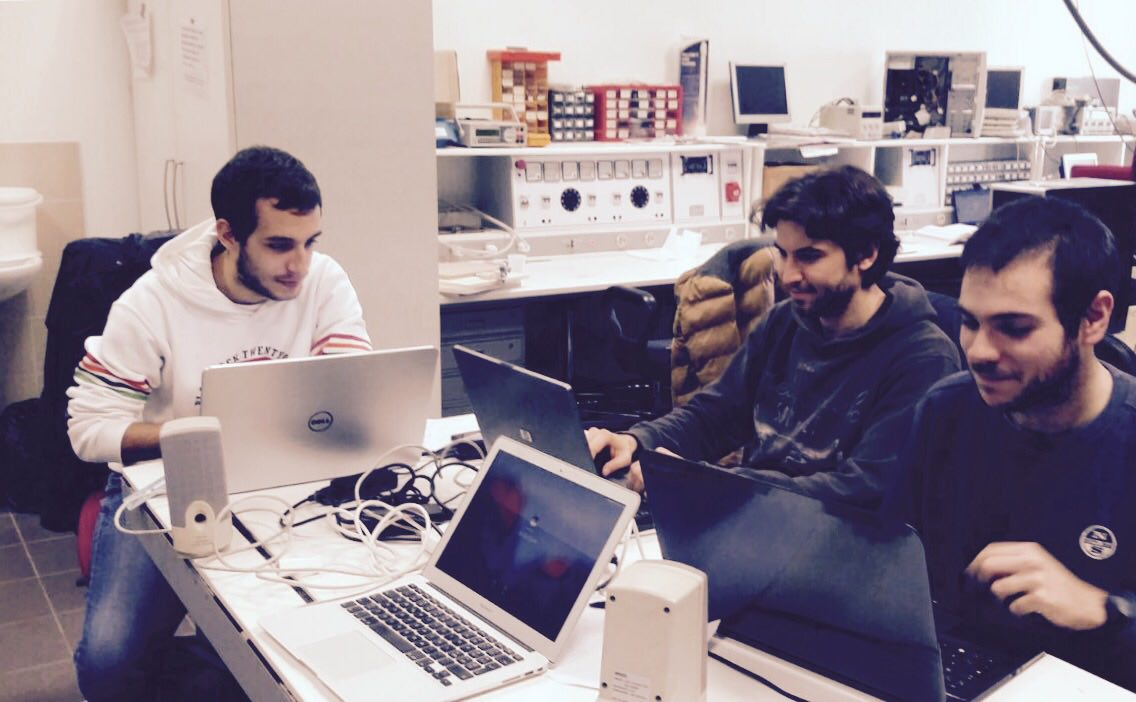
\includegraphics[width=\textwidth]{images/team}
\caption{Il team di sviluppo del Progetto Heimdall durante i test del web switch a pieno regime (\emph{febbraio 2016, Laboratori di Tor Vergata})}
\end{figure}
\end{document}